%\documentclass[linenumbers,trackchanges]{aastex701}
\documentclass[preprint]{aastex701}
\usepackage[utf8]{inputenc}
\usepackage{graphicx} % Required for inserting images
\usepackage{amssymb}
\usepackage{todonotes}
\usepackage{comment}

\graphicspath{{Figure/}}

\newcommand{\hinvMpc}{h^{-1}{\rm Mpc}}

\newcommand{\ZZ}[1]{{\color{red} [ZZ: #1]}}

\begin{document}

\title{Studying Matter Distribution around Pairs of Dark Matter Halos from Cosmic Microwave Background Lensing}

\author[]{Caroline Wu}
\affiliation{Scarsdale High School, 1057 Post Road, Scarsdale, NY 10583}
\email[show]{carolinewu327@gmail.com}

\begin{abstract}
Dark matter distribution around pairs of dark matter haloes encodes information about the gravitational interaction between haloes and probes the associated filamentary structure. In this work, we use the BOSS CMASS galaxy sample and Planck 2018 cosmic microwave background (CMB) lensing map to study the matter distribution around galaxy pairs. We produce stacked CMB lensing $\kappa$ maps around galaxy pairs, in transverse pair separation bins centered
at $5$, $10$, and $20\,\hinvMpc$. With comparison to the maps from control pairs, obtained by superposition of $\kappa$ distribution around single galaxies, a quadrupole pattern in the matter distribution around galaxy pairs is revealed for the first time, with excess around the pair connection line and deficit around the perpendicular bisector. Such a pattern is consistent with the expectation from cosmological $N$-body simulations, pointing to an origin from tidal interaction. There is hint of matter excess in between galaxy pairs, associated with filaments, and an increased galaxy pair sample and/or CMB lensing reconstruction with improved precision would be necessary for a firm detection.

\begin{comment}
We search for gravitational lensing associated with cosmic-web filaments by
stacking the Planck 2018 CMB lensing convergence map on pairs of BOSS CMASS
galaxies at $z\simeq0.55$. We stack pairs on a fixed comoving grid, without
rescaling them to a common separation, in transverse-separation bins centered
at $5$, $10$, and $20\,\hinvMpc$. We subtract a unit-amplitude control formed
by placing the observed single-galaxy profile at the two galaxy positions and
define the bridge excess as the difference between a central band along the
pair axis and two flanking bands. This residual can also contain differences
between the halo and environmental signals of paired and average galaxies. We
combine the North and South Galactic caps and estimate the profile covariance
with a $287$-region spatial jackknife. Applying the same signal estimator to a
CMASS-like BigMDPL mock predicts bridge excesses of
$(6.3,\,4.9,\,2.2)\times10^{-4}$ at these separations. The observed bridge
excesses are $(5.4\pm9.1,\,11.9\pm5.1,\,1.2\pm2.2)\times10^{-4}$, corresponding to
$0.6\sigma$, $2.3\sigma$, and $0.6\sigma$. No bridge excess exceeds
$3\sigma$, and all three measurements are consistent with both zero and the
mock prediction. The predicted amplitudes are smaller than the observational
errors at every separation. Resolving their separation dependence requires a
lower-noise convergence map.
\end{comment}

\begin{comment}
We search for the lensing signal of cosmic-web filaments by stacking the
Planck CMB lensing convergence map on pairs of BOSS CMASS galaxies. Unlike
previous pair-stacking work, we do not rescale pairs to a common separation:
we stack on a fixed physical grid in three separation bins centred at 5, 10,
and 20 $h^{-1}$ Mpc, so the residual can be tracked as a function of halo
separation. The two halos are removed with a control map built from the
observed single-galaxy stack, decomposed into a compact core and an extended
tail whose amplitudes are fitted outside the pair. Every choice in the
estimator was fixed beforehand in a matched simulation, built from BigMDPL
halos populated to reproduce the CMASS number density. North and South are
stacked as one joint sample, and uncertainties come from a 287-region spatial
jackknife in which every fitted parameter is re-fitted. We measure bridge
convergences of $(1.74 \pm 11.29)$, $(8.94 \pm 7.45)$, and
$(4.39 \pm 4.60) \times 10^{-4}$ at the three separations, or $0.15\sigma$,
$1.20\sigma$, and $0.95\sigma$. We therefore do not detect a filament signal.
The expected quadrupole pattern is visible in the difference maps and matches
the simulation in amplitude, and the control passes its null tests, but the
uncertainty is set almost entirely by noise in the Planck map: repeating the
measurement with no control at all changes the error by less than 7\%. The
simulation predicts a bridge below our noise level, so this null is the
expected outcome rather than a tension.
\end{comment}
\end{abstract}

\keywords{\uat{Galaxies}{573} --- \uat{Cosmology}{343}}

\section{Introduction}

\label{sec:intro}

On scales of tens of megaparsecs the matter distribution of the Universe is
organized into a cosmic web of nodes, filaments, sheets, and voids. Anisotropic
gravitational collapse provides a simple origin for this hierarchy: in the
Zel'dovich approximation, one-axis collapse produces sheets, whereas two-axis
collapse produces filaments
\citep{Zeldovich1970, BondKofmanPogosyan1996}.
The NEXUS+ classification of an $N$-body simulation assigns roughly half of
the matter to filaments, which occupy about 6 percent of the volume
\citep{Cautun2014}. Filaments may also contain much of the baryonic matter
not accounted for by stars, cold gas, and the hot atmospheres of groups and
clusters. Low-redshift censuses have historically left roughly 30 percent of
the cosmic baryon budget unaccounted for \citep{FukugitaHoganPeebles1998,
Shull2012}, while hydrodynamic simulations place a substantial baryon
fraction in a warm--hot intergalactic medium at
$T\sim10^{5}$--$10^{7}\,\mathrm{K}$ that traces the filamentary web
\citep{CenOstriker1999}. Measurements of filament matter test structure
formation and provide a gravitational reference for studies of filament gas,
but lensing alone does not determine the baryon fraction
\citep{deGraaff2019, Tanimura2020, Nicastro2018}.

Gravitational lensing traces projected mass irrespective of its composition.
For a spatially flat universe with sources at comoving distance $\chi_{\rm s}$,
the convergence in direction $\hat{\boldsymbol n}$ is
\begin{equation}
  \kappa(\hat{\boldsymbol n}) = \int_{0}^{\chi_{\rm s}} \mathrm{d}\chi\,
  W(\chi)\,\delta(\chi\hat{\boldsymbol n},\chi), \qquad
  W(\chi) = \frac{3\Omega_{\rm m}H_{0}^{2}}{2c^{2}}\,
  \frac{\chi}{a(\chi)}\,\frac{\chi_{\rm s}-\chi}{\chi_{\rm s}},
  \label{eq:kappa}
\end{equation}
where $\chi$ is comoving distance and $a$ is the scale factor
\citep{Bartelmann2001}. For a selected sample of filament candidates, $\kappa$
probes the associated matter without converting galaxy counts through a bias
model or assuming a thermodynamic state for the gas.
Equation~(\ref{eq:kappa}) also
sets the scale of the expected signal. For a source at the last-scattering
surface, $z_{\rm s}\simeq1090$, the kernel $W(\chi)$ is broad and peaks near
$z\sim2$ \citep{LewisChallinor2006}; at the redshift of the BOSS CMASS sample,
$z\simeq0.55$, its value is $W\simeq7\times10^{-5}\,\mathrm{Mpc}^{-1}$.
An idealized filament with overdensity $\delta\sim3$--$5$ and a comoving
line-of-sight depth of a few megaparsecs then produces
$\kappa\sim(0.5$--$1.5)\times10^{-3}$ \citep{Colberg2005}. For a lens at
$z\simeq0.55$, a
background galaxy population at $z_{\rm s}\sim1$ has lower lensing efficiency
than the CMB. Although intrinsic source shapes add noise, deep galaxy imaging
provides much finer angular resolution and can achieve high statistical
precision over a smaller footprint.

The lensing signal of a filament usually requires the stacking of many candidate structures. Candidates may be identified algorithmically from
the galaxy distribution or, as in this work, defined by pairs of massive
galaxies whose connecting axis sets the expected orientation of a bridge. In
an $N$-body study of cluster-mass haloes, all pairs separated by less than
$5\,\hinvMpc$ were connected by a filament, compared with roughly one third
at $15$--$20\,\hinvMpc$ \citep{Colberg2005}.
CMASS galaxies occupy haloes of $M\sim10^{13}\,h^{-1}\mathrm{M}_{\odot}$
\citep{White2011}, so a pair at these separations is a plausible filament
anchor. The mean convergence around such a pair contains the one-halo
profiles of the two members, matter in their correlated environments, and an
anisotropic excess along the axis joining them. In correlation-function
language, subtracting the superposed galaxy--matter two-point contributions
is intended to isolate the connected galaxy--galaxy--matter three-point term
\citep{Clampitt2016}. An empirical control cannot perform this separation
exactly, because paired galaxies occupy different environments from average
galaxies. We therefore refer to the control-subtracted field as a residual
and interpret its axial excess as filament-associated rather than as a pure
filament map. The mock predicts that this excess decreases with pair
separation, reflecting changes in both the connected-pair fraction and the
matter distribution around the pairs. And so, a primary goal of this work is to measure this dependence.

Two selection effects are especially important for pair purity. Projection
pairs galaxies that are close on the sky but distant along the line of sight;
these unconnected pairs dilute the mean signal. Relative peculiar velocities
also perturb radial separations inferred from redshifts. For halo pairs on
these scales, the relative line-of-sight velocity has a dispersion of
$\sigma_{v}\simeq500\,\mathrm{km\,s^{-1}}$
\citep{Jenkins1998, deGraaff2019}. At $z=0.55$ this
corresponds to a comoving displacement $(1+z)\sigma_{v}/H(z)\simeq
6\,\hinvMpc$, which is why previous pair-stacking analyses have adopted a
line-of-sight cut of $5$--$6\,\hinvMpc$. Such a cut rejects some genuinely
connected pairs whose members have large relative velocities and admits some
unconnected pairs that happen to lie within the velocity window, but it
retains pairs whose axes are close to the plane of the sky, minimizing
line-of-sight dilution of the bridge.

\subsection{Previous stacked lensing measurements of filaments}

Existing measurements divide according to whether the lensing source is a
population of background galaxies or the CMB.

\citet{Clampitt2016}, \citet{EppsHudson2017}, and \citet{Kondo2020} use galaxy
shapes. \citet{Clampitt2016} measured the stacked shear around pairs of SDSS luminous red galaxies at $z\approx0.25$ with projected separations of
$6$--$14\,\hinvMpc$ and line-of-sight separations below $6\,\hinvMpc$, using
SDSS source shapes over approximately $8000\,\mathrm{deg}^{2}$, and reported
a $4.5\sigma$ detection. Their four-point shear estimator uses symmetry to
cancel the signal of two spherical haloes and isolate the bridge.
\citet{EppsHudson2017} stacked the weak-lensing signal from CFHTLenS source
shapes around BOSS LOWZ and CMASS pairs at a mean redshift
$\langle z\rangle\approx0.42$. While their pairs pairs had the same projected
separation, this was paired with a larger line-of-sight separation as a control and reported a
$5\sigma$ excess after subtracting this control from the physical-pair
stack. \citet{Kondo2020} paired BOSS CMASS galaxies at $z\approx0.55$ with
first-year Subaru Hyper Suprime-Cam shapes. Although
the overlap footprint is only $\sim140\,\mathrm{deg}^{2}$ and contains
$14{,}422$ CMASS galaxies, the source density of $\sim22\,\mathrm{arcmin}^{-2}$
yielded a $3.9\sigma$ detection. Their mock analysis showed that intrinsic
variation among filaments together with projected large-scale structure
contributes about 60 percent of the covariance, with source shape noise
contributing the remaining 40 percent.

The CMB provides a complementary source. Its lensing kernel is broad, the
reconstruction is free of galaxy shape noise and intrinsic alignments, and
the Planck maps cover most of the sky, so the full BOSS footprint can be
used. However, the Planck reconstruction is strongly noise dominated on the
angular scales relevant to these filaments \citep{Planck2018lensing} and may
retain foreground contamination. Two earlier studies used filaments
identified directly from the spectroscopic galaxy distribution.
\citet{He2018} applied a density-ridge algorithm to the CMASS
distribution \citep{Chen2016}, constructed a filament intensity map from the
resulting catalog, and cross-correlated it with the Planck convergence map,
obtaining a $5\sigma$ detection and a filament bias $b_{\rm f}\approx1.5$.
\citet{Tanimura2020} identified $24{,}544$ filaments of length
$30$--$100\,\mathrm{Mpc}$ in LOWZ+CMASS with DisPerSE \citep{Sousbie2011},
masked the critical points at their ends, and stacked Planck $\kappa$ on the
filament spines, reaching $8.1\sigma$. We cannot compare these significances directly to the pair-stacking results. These studies identify longer structures
directly from the galaxy density field and use different estimators, whereas
a pair sample includes unconnected pairs that dilute the mean.

The study of \citet{deGraaff2019} is the closest predecessor of this work.
Their primary measurement was the thermal Sunyaev--Zel'dovich signal of
filament gas, and they applied the same pipeline to the Planck convergence
map to estimate the filament matter density. They stacked around
$1{,}002{,}334$ pairs
drawn from the BOSS CMASS catalog used here, with transverse comoving
separations of $6$--$14\,\hinvMpc$ and line-of-sight separations below
$5\,\hinvMpc$. Each pair was rotated to a common orientation, rescaled to unit
separation, projected onto a rectangular grid, and reflected to exchange the
two members. Halo contributions were removed by fitting an isotropic radial
profile within a $60^{\circ}$ cone perpendicular to the pair axis and
subtracting the resulting two-dimensional model. Because the convergence map
was matched to the $10$-arcmin resolution of the Compton-$y$ map, the
lensing analysis also used $10$-arcmin smoothing. They measured a mean
filament convergence of
$\bar{\kappa}=(0.58\pm0.31)\times10^{-3}$ between the pair members, a
$1.9\sigma$ result. The significance increased to $3.1\sigma$ when the region
beyond the pair was included.

\subsection{This work}

We revisit the combination of BOSS CMASS pairs with Planck CMB lensing,
following \citet{deGraaff2019}, with four changes in design.

First, we resolve the measurement in pair separation rather than integrating
over it. Whereas \citet{deGraaff2019} rescaled every pair to a normalized
separation before stacking, we stack on a fixed comoving grid of
$101\times101$ pixels spanning $100\times100\,(\hinvMpc)^{2}$, using disjoint
separation bins centered at $5$, $10$, and $20\,\hinvMpc$. The finite bin
width causes some smearing, but the construction allows us to test
the predicted decline of the anisotropic excess with separation described
above.

Second, we apply the signal estimator to a simulation. We construct a
CMASS-like mock catalog from the BigMDPL $N$-body simulation
\citep{Klypin2016} and apply matched pair selection, smoothing, stacking,
control subtraction, and fixed-band measurement to a convergence map from the
same volume. This provides a separation-dependent $\Lambda$CDM reference for
the amplitude and transverse profile of the residual, measured with the same
statistic as the observed stacks.

Third, we use a different halo-subtraction method. Where
\citet{deGraaff2019} fit an isotropic profile to the observed pair stack
itself, we subtract a control map built by displacing the stack of single
CMASS galaxies to $\pm d/2$ along the pair axis, in the spirit of the control
stacks of \citet{EppsHudson2017}. Profile fitting can absorb part of the
bridge into the halo model. Our control instead models the one-halo and
isotropic environmental terms using the profile of an average CMASS galaxy.
Galaxies selected to have a close companion reside in different environments,
so this profile need not match the halo and environmental contributions
around paired galaxies. The subtraction can therefore leave both isotropic
and axis-aligned residuals that cannot be assigned uniquely to a filament.
We apply the same control to the mock and compare the resulting residual,
rather than an isolated filament component, with the data.

Fourth, we vary the line-of-sight cut rather than adopting the
$5$--$6\,\hinvMpc$ value used in previous pair-stacking studies. Larger cuts
increase the pair count but admit more unconnected pairs, and, as discussed
above, peculiar velocities of $\sim500\,\mathrm{km\,s^{-1}}$ move pairs across
any threshold of a few $\hinvMpc$. We therefore measure directly how the cut
trades completeness against contamination, using the mock to identify
interlopers in real space.

We use the Planck 2018 minimum-variance lensing reconstruction
\citep{Planck2018lensing} synthesized at $N_{\rm side}=2048$ and smoothed with
an $8$-arcmin Gaussian kernel, compared with the $10$-arcmin smoothing of
\citet{deGraaff2019}. At $z=0.55$ the comoving distance is
$\chi\simeq1400\,\hinvMpc$, so $8$ arcmin corresponds to $\simeq3.3\,\hinvMpc$,
comparable to the few-megaparsec transverse width of inter-halo filaments
\citep{Colberg2005}. Pair separations of $5$, $10$, and $20\,\hinvMpc$ subtend
approximately $12$, $24$, and $48$ arcmin. The smallest separation spans only
about 1.5 beam widths, so its bridge profile is poorly resolved and its
central bin can contain beam-convolved halo residuals.

Throughout we adopt the Planck 2018 cosmology with $h=0.6766$ and quote
comoving distances in $\hinvMpc$. We use ``filament-associated signal'' for a
positive axial convergence excess between the pair members. We use
``residual'' for the full control-subtracted field because it can also contain
imperfectly subtracted halo and environmental contributions.

The paper is organized as follows. Section~\ref{sec:data} describes the
CMASS and random catalogs, the Planck lensing map, and the BigMDPL mock
catalog with its simulated convergence map. Section~\ref{sec:method}
presents the pair selection, stacking, control construction, band statistic,
and error estimation for the data and mock.
Section~\ref{sec:sim_expect} gives the $\Lambda$CDM reference signal from the
mock. Section~\ref{sec:results} reports the observed stacks, the bridge
convergence at each separation, the comparison with the mock prediction and
with previous work, and the robustness tests. Section~\ref{sec:discussion}
summarizes the results and discusses their implications.


\begin{comment}
The paper is organised as follows. Section~\ref{sec:data} describes the
CMASS and random catalogues and the Planck lensing map.
Section~\ref{sec:method} presents the pair selection, stacking, control
construction, and error estimation. Section~\ref{sec:mocks} describes the
BigMDPL mock catalogue and the simulated convergence maps.
Section~\ref{sec:results} reports the stacked maps, the separation and
line-of-sight dependence of the residual signal, and the comparison with the
mock prediction. Section~\ref{sec:discussion} discusses systematics and the
implications for the matter content of filaments, and
Section~\ref{sec:conclusions} concludes.
}

\todo[inline]{
Previous stacked weak-lensing measurements of cosmic-web filaments can be divided broadly according to whether they use background galaxies or the CMB as the lensing source.

Clampitt et al. (2016), Epps \& Hudson (2017), and Kondo et al. (2020) fall into the first category, which uses galaxy shapes as the source. Clampitt et al. (2016) stacked the shear field around pairs of SDSS luminous red galaxies at $z\approx0.25$, selecting projected separations of $6$--$14\,\hinvMpc$ and line-of-sight separations below $6\,\hinvMpc$. Approximately $8000\,\mathrm{deg}^{2}$, they reported a $4.5\sigma$ detection. They used a four-point estimator that analytically cancels the tangential-shear contribution of the two spherically symmetric host halos, isolating the bridge between them. Using CFHTLenS source shapes, Epps \& Hudson (2017) studied the BOSS LOWZ and CMASS pairs at a mean redshift of $\langle z\rangle\approx0.42$. They reported a $5\sigma$ excess after subtracting the convergence stack of non-physical pairs from that of physical pairs.Kondo et al. (2020) paired BOSS CMASS galaxies at z $\approx$ 0.55 with first-year Subaru Hyper Suprime-Cam shapes. Despite an overlap footprint of only ~140 degrees squared containing 14,422 CMASS galaxies, the depth of HSC imaging yielded a 3.9 sigma detection. Their mock analysis showed that intrinsic variation between filaments and projected large-scale structure contributed approximately 60\% of the covariance, with source shape noise contributing the remainder.

A complementary approach uses the CMB as the background source. The CMB source plane lies at $z_\ast\simeq1090$, and its broad lensing kernel probes matter over a wide redshift range. CMB lensing avoids galaxy shape noise and intrinsic alignments and is available over a large fraction of the sky, but the Planck reconstruction has substantial reconstruction noise, limited angular resolution, and possible foreground-related systematics.Other studies have measured CMB lensing associated with filaments identified directly from the spectroscopic galaxy distribution. He et al. (2018) identified filaments directly with a density-ridge algorithm applied to the CMASS distribution, built an intensity map from the resulting ridge catalog, and cross-correlated it with the Planck convergence map, obtaining $5\sigma$. Tanimura et al. (2020) took a similar approach with DisPerSE, stacking Planck $\kappa$ on 24,544 filaments of length 30-100 Mpc identified in LOWZ+CMASS and reaching $8.1\sigma$ in convergence. These significances are not directly comparable to pair-stacking measurements because the studies probe longer, differently selected structures and use different estimators; pair selection can also dilute the mean signal when candidate pairs are not physically connected.

The study by de Graaff et al. (2019) is the closest predecessor to this work. They stacked a Planck CMB-lensing convergence map around pairs drawn from the same parent BOSS CMASS catalogs used here. They selected 1,020,334 pairs with transverse comoving separations of $6$--$14\, \hinvMpc$ and line-of-sight separations below $5\,\hinvMpc$. Their pipeline rotates each pair to a common orientation, rescales it to a normalized separation, projects the surrounding map onto a rectangular grid, and reflects each cutout to exchange the two pair members. Halo contributions are removed by fitting an isotropic radial profile within a 60 degree cone perpendicular to the pair axis and subtracting the resulting 2D model. They measured a mean filament convergence of $\kappa = (0.58 \pm 0.31) \times 10^{-3}$, corresponding to a marginal $1.9\sigma$ detection. 

We do not claim a novel class of data combination: de Graaff et al. previously
combined BOSS CMASS pairs with a Planck CMB-lensing reconstruction. Our analysis differs from theirs in several aspects. 

First, we resolve the measurement in pair separation rather than integrating over it. While de Graaff rescales every pair to a normalized separation before stacking, we stack on a fixed comoving grid of $101\times101$ pixels spanning $100\times100\, (\hinvMpc)^2$, using disjoint separation bins centered at $5$, $10$, and $20\, \hinvMpc$. Although the finite width of each bin modestly smears the bridge, this construction allows us to measure the separation dependence of the residual signal.

Second, we model the entire measurement in simulation. We construct a CMASS-like mock catalog from BigMDPL and apply matched pair selection, map smoothing, stacking, and halo-subtraction operations to the simulated convergence maps. This provides a separation-dependent $\Lambda$CDM reference that can be compared directly with the observed stacks.

Third, we use an independent halo-subtraction method. Where de Graaff et al. fit an isotropic profile to the observed stack itself, we subtract a control map built by displacing the single-galaxy stack to $\pm d/2$ along the pair axis, following the spirit of Epps \& Hudson (2017). The methods have different weaknesses: profile fitting can remove part of the bridge, while control subtraction may not accurately represent paired galaxies. 

Fourth, we test different line-of-sight cuts instead of adopting the 5-6 $\hinvMpc$ cut used in previous pair-stacking studies. Larger cuts increase the sample size but also admit more unassociated pairs, while peculiar velocities can move pairs across the threshold. We therefore measure how the cut affects the contamination and the recovered signal. 

We use the Planck 2018 minimum-variance lensing reconstruction at $N_{\rm side} =2048$ and apply an $8$-arcmin Gaussian smoothing kernel, rather than the $10$-arcmin smoothing adopted by de Graaff et al. This is a modest resolution difference because the reconstruction remains noise dominated on small angular scales.
\todo[inline]{
in this work, CMB lensing, directly probe the convergence $\kappa$ or the surface matter density around galaxy pairs

structure of this paper}
\end{comment}

\section{Data}
\label{sec:data}

The observational measurements of the matter distribution around galaxy pairs combine three ingredients: spectroscopic galaxy positions
from BOSS, which define the pairs and the single-galaxy control; the
corresponding BOSS random catalogs, which trace the angular selection and
measure footprint-dependent offsets; and the Planck CMB lensing convergence
map, from which we construct the galaxy and random stacks. An $N$-body mock
of the CMASS sample and the corresponding  convergence field provide a $\Lambda$CDM
reference model
(Section~\ref{sec:sim}), which guides observational measurements and aids interpretation.

\subsection{BOSS CMASS galaxies}
\label{sec:data_cmass}

Galaxy positions come from the CMASS sample of the Baryon Oscillation
Spectroscopic Survey \citep[BOSS;][]{Dawson2013}, part of SDSS-III
\citep{Eisenstein2011}, in its twelfth data release
\citep{Alam2015, Reid2016}. CMASS targets were selected with color and
magnitude cuts designed to follow a passively evolving stellar-population
locus, so that the sample has an approximately constant stellar mass across
its redshift range (hence the name). The galaxies are luminous red galaxies
hosted by haloes of typical mass $M\simeq10^{13}\,h^{-1}\mathrm{M}_{\odot}$,
with a satellite fraction of about 10 percent \citep{White2011}. 
%Massive hosts are useful here because their one-halo lensing signal can be measured and modeled, and 
Simulations predict that pairs of such haloes are often connected by filaments \citep{Colberg2005}.

We use data from both Galactic caps, referred to as North and South, and restrict the sample to $0.4<z<0.7$, slightly wider than the $0.43<z<0.7$ range
adopted for the BOSS clustering analyses \citep{Reid2016}.
% CHECK: document the reason for using 0.4 rather than 0.43.
After this cut the sample contains $792{,}294$ galaxies, $579{,}089$ in the
North and $213{,}205$ in the South.  
%with a summed weight of $847{,}528$.
The effective survey area is approximately $6{,}850\,\mathrm{deg}^{2}$ in the
North and $2{,}525\,\mathrm{deg}^{2}$ in the South, for a total of
$9{,}376\,\mathrm{deg}^{2}$ \citep{Reid2016}. % CHECK against Reid+2016 Table 2
Figure~\ref{fig:footprint_zdist} shows the footprint of both caps together
with the Planck lensing mask. The sample has a median redshift of $z=0.539$
%and a weight-averaged redshift of $\langle z\rangle=0.545$; 
and galaxies in the two caps have very similar redshift distributions.

Each galaxy carries the standard BOSS systematic weights
\citep{Ross2012, Reid2016}. We combine them as
\begin{equation}
  w = w_{\rm seeing}\, w_{\rm star}\,
      \left(w_{\rm noz} + w_{\rm cp} - 1\right),
  \label{eq:weights}
\end{equation}
where $w_{\rm seeing}$ and $w_{\rm star}$ correct the angular selection
function for variations in seeing and stellar density, $w_{\rm cp}$ accounts
for close pairs lost to fiber collisions, and $w_{\rm noz}$ accounts for
redshift failures. We do not apply the FKP weight because it is designed to
optimize clustering measurements rather than the stacking estimator in this work.

% CHECK: quantify the effect of removing the Sigma_crit weight from the
% single-galaxy stacks (weighting_sensitivity.py).

We transform right ascension and declination into Galactic longitude and
latitude $(l,b)$, the native frame of the Planck maps, and turn redshifts
into comoving distances under the Planck 2018 cosmology
\citep{Planck2018lensing}, quoted in $\hinvMpc$ with $h=0.6766$. 
%: every galaxyenters with its own weight, so the relative contribution of the two caps is set by their galaxy content rather than by a separate average (Section~\ref{sec:method}).

\begin{figure}
  \centering
  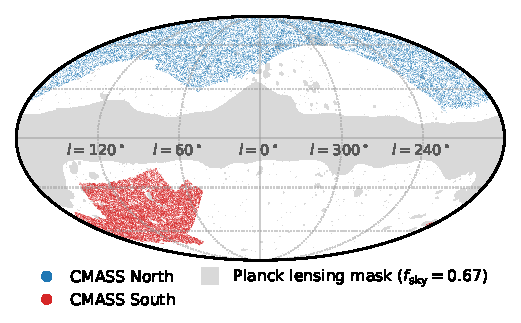
\includegraphics[width=0.48\linewidth, trim=0 -3cm 0 0]{footprint.pdf}
  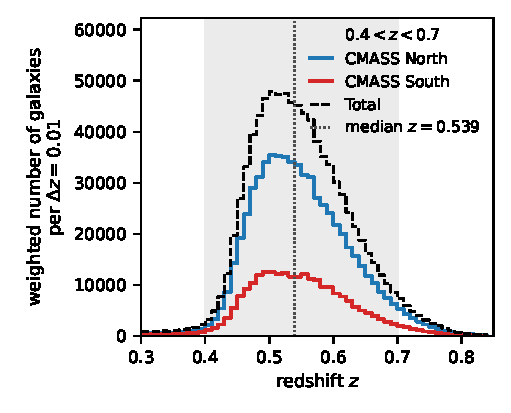
\includegraphics[width=0.48\linewidth]{zdist.pdf}
  \caption{Left: footprint of the BOSS CMASS North and South samples in
  Galactic coordinates, overlaid on the Planck 2018 lensing analysis mask.
  Right: weighted redshift distribution of the CMASS galaxies in each cap
  and in total, with the $0.4<z<0.7$ selection shaded and the median
  redshift of the selected sample marked.
  
  \label{fig:footprint_zdist}
\end{figure}

\subsection{Random catalogs}
\label{sec:data_random}

The BOSS random catalogs \citep{Reid2016} sample the angular selection
function of each cap at roughly fifty times the galaxy density, with
redshifts assigned from the observed galaxy distribution. The randoms
therefore share the galaxies' redshift distribution $n(z)$ but contain no clustering. We apply the
same $0.4<z<0.7$ cut and use the full catalogs, $40.9$ million points over
both caps, for every random stack. 
%Replacing the full catalog by a 10 percent subsample shifts the $10\,\hinvMpc$ bridge excess by $5\times10^{-4}$, comparable to the measured signal.
% CHECK: combine_filament_jackknife.py docstring.
Random points carry unit systematic weight and, in the single-galaxy stacks,
the same lensing-efficiency weight as the galaxies.

The randoms serve three purposes. First, a stack of the convergence map
around random points measures the mean convergence of the footprint,
including any residual mean-field or mask-related offset, and is subtracted
from the single-galaxy stack. Second, pairs of random points selected with
the same separation criteria as the galaxy pairs provide the equivalent
correction for the pair stack. Because the number of random pairs is of
order $10^{9}$, the full random catalog is needed to reduce the noise in this
correction. Third, a seeded 10 percent subsample of the randoms traces the
survey footprint on a coarse HEALPix grid to define the jackknife regions
used for error estimation (Section~\ref{sec:method}).

\subsection{Planck CMB lensing map}
\label{sec:data_planck}

We use the Planck 2018 lensing reconstruction \citep{Planck2018lensing},
release \texttt{COM\_Lensing\_4096\_R3.00}. The convergence harmonic
coefficients $\kappa_{LM}$ are taken from the minimum-variance combination
of the temperature and polarization quadratic estimators applied to the
SMICA foreground-cleaned maps. The Planck pipeline subtracts the estimator
mean field, and the coefficients are provided up to
$L_{\rm max}=4096$. As discussed in Section~\ref{sec:intro}, the
reconstruction is noise dominated on the small angular scales relevant to
this work.

We produce a HEALPix \citep{Gorski2005} $\kappa$ map with $N_{\rm side}=2048$, corresponding to a pixel scale of $1.7\,\mathrm{arcmin}$, smoothed with a Gaussian beam of $8\,\mathrm{arcmin}$ full width at half maximum (FWHM).
%Before stacking we multiply $\kappa_{LM}$ by a Gaussian beam of $8\,\mathrm{arcmin}$ full width at half maximum (FWHM) and synthesize a HEALPix map \citep{Gorski2005} at $N_{\rm side}=2048$, corresponding to a pixel scale of $1.7\,\mathrm{arcmin}$. 
The smoothing suppresses small-scale reconstruction
noise. At $z=0.55$, $8\,\mathrm{arcmin}$ spans
$\simeq3.3\,\hinvMpc$ comoving. 
%Section~\ref{sec:robust} compares this fiducial choice with the available $4$- and $6$-arcmin results. 
%We sample the smoothed map at the sky positions corresponding to the comoving stack grid by nearest-pixel lookup, without interpolation.

We apply the Planck lensing analysis mask distributed with the release,
which removes the Galactic plane, point sources, and regions of poor
foreground cleaning and retains 67.1 percent of the sky. %Masked pixels receive zero weight in every stack, so that the stacked value at each grid position is a weighted mean over unmasked pixels only. 
The CMASS footprint lies almost entirely within the unmasked region: 96.5 percent of North and 94.7 percent of South galaxies, 96.0 percent overall, fall on unmasked
pixels (Fig.~\ref{fig:footprint_zdist}). 
%The remainder lie mostly in the point-source and cluster holes of the mask and at the low-latitude edge of the North cap (Fig.~\ref{fig:footprint_zdist}).
% CHECK: the fraction whose full 100 h^-1 Mpc cutout is unmasked is not yet computed.

\subsection{$N$-body simulation and mock galaxy catalog}
\label{sec:sim}

For a $\Lambda$CDM reference model we build a mock galaxy catalog from
BigMDPL, an $N$-body cosmological simulation in the MultiDark suite
\citep{Klypin2016, Riebe2013}. BigMDPL follows $3840^{3}$ dark-matter
particles of mass $2.36\times10^{10}\,h^{-1}\mathrm{M}_{\odot}$ in a periodic
box of comoving side $2500\,\hinvMpc$; its cosmology has
$\Omega_{\rm m}=0.307$ and $h=0.678$. We work with the $a=0.6464$ output, at
$z=0.547$, the snapshot nearest the weighted mean redshift of CMASS. Halos
come from the public Rockstar catalog, from which we retain hosts and drop
subhaloes, adopting the Rockstar virial mass $M_{\rm vir}$. 
%The HOD is applied to hosts with $\log_{10}(M_{\rm vir}/h^{-1}\mathrm{M}_{\odot})\geq12.5$.

We assign galaxies to haloes above $\log_{10}(M_{\rm vir}/h^{-1}\mathrm{M}_{\odot})=12.5$ within the halo occupation distribution (HOD) framework. 
The mean occupation function of central galaxies follows a form for CMASS galaxies in \citet{White2011},
%Mock galaxies are placed with a central-only halo occupation distribution (HOD) of the form adopted for CMASS by \citet{White2011},
\begin{equation}
  \langle N_{\rm cen}(M)\rangle = \frac{1}{2}\left[1+\mathrm{erf}
  \left(\frac{\ln(M/M_{\rm cut})}{\sqrt{2}\,\sigma}\right)\right],
  \label{eq:hod}
\end{equation}
with $\sigma=0.94$. We set the cutoff mass scale $\log_{10}(M_{\rm cut}/h^{-1}\mathrm{M}_{\odot})=13.246$ to match the CMASS central-galaxy number density,
$2.70\times10^{-4}\,h^{3}\,\mathrm{Mpc}^{-3}$: the observed density of
$3\times10^{-4}\,h^{3}\,\mathrm{Mpc}^{-3}$ multiplied by a central fraction
of 0.9.
%We use $\log_{10}(M_{\rm cut}/h^{-1}\mathrm{M}_{\odot})=13.246$, rather than the value $13.04$ adopted by \citet{White2011}. With our halo definition and catalog mass floor, the latter gives a number density of $4.21\times10^{-4}\,h^{3}\,\mathrm{Mpc}^{-3}$. We set the threshold to match the CMASS central-galaxy density, $2.70\times10^{-4}\,h^{3}\,\mathrm{Mpc}^{-3}$: the observed density of $3\times10^{-4}\,h^{3}\,\mathrm{Mpc}^{-3}$ multiplied by a central fraction of 0.9.
% Provenance: analysis/sim/results/galaxies_hod_nmatch.csv.meta.json
% (run 2026-07-20, occupation seed 20260720). 13.246 solves nbar = 0.9 * 3e-4
% over hosts_minmass12p5.bin; make_hod_catalog.py still defaults to the
% published White+11 value 13.04, so the paper run passes --log10-mcut.
%Each host receives a galaxy with probability $\langle N_{\rm cen}\rangle$.
%The input halo catalog ends at the stated mass floor, where the adopted
%occupation is still $0.034$, and therefore truncates the low-mass tail of
%the model. 
The mock contains no satellites, whereas about 10 percent of
CMASS galaxies are satellites \citep{White2011}; we return to this limitation
in Section~\ref{sec:discussion}. 
%Halo peculiar velocities are included in the redshift-space pair selection.

We choose the line-of-sight direction as one principal axis to put the mock galaxy catalog in redshift space. That is, the line-of-sight position of each galaxy is shifted by $(1+z)\,v_{\parallel}/H(z)$, with $v_{\parallel}$ denoting the line-of-sight peculiar-velocity of the host halo and $H(z)$ being the Hubble parameter at redshift $z$. 

%The second halo sample used for the sensitivity tests consists of hosts within $\pm0.05$ dex of $\log_{10}(M_{\rm vir}/h^{-1}\mathrm{M}_{\odot})=13.0$ (Section~\ref{sec:method}).

For the simulated convergence map, we make use of the 0.5 percent randomly sampled particles of the simulation, with $N_{\rm tot}=2.8\times10^{8}$ particles in total.
%The simulated convergence map is built from the public 1-in-200 particle subsample, which contains $2.8\times10^{8}$ particles. Each sampled particle has an effective mass equal to 200 simulation particles. 
We project the particles along the chosen principal axis of the simulation box 
%through the full $2500\,\hinvMpc$ depth 
onto a periodic 2-dimensional (2D) grid with pixel width $0.1\,\hinvMpc$. For each pixel, we calculate the mean-subtracted surface density as
\begin{equation}
    \Sigma(\mathbf{x})=m_{\rm eff}\left[\frac{N_{\rm p}(\mathbf{x})}{\ell^{2}}
-\frac{N_{\rm tot}}{L^{2}}\right],
\end{equation}
where $N_{\rm p}(\mathbf{x})$ is the number of particles in the pixel of width $\ell$, and $N_{\rm tot}$ is the total number particles in the box of size $L$, and $m_{\rm eff}$ is the effective mass of each particle in the subsample (i.e., 200 times the particle mass in the simulation). We convert the surface density to convergence as $\kappa=\Sigma/\Sigma_{\rm crit}$ with the comoving critical density for a lens at $z=0.547$ and the CMB as source, $\Sigma_{\rm crit}=8.88\times10^{14}\,h\,\mathrm{M}_{\odot}\,\mathrm{Mpc}^{-2}$.
Similar to the CMB lensing map, the simulation$\kappa$ map is smoothed with a periodic two-dimensional Gaussian kernel of FWHM $3.31\,\hinvMpc$, corresponding to $8\,\mathrm{arcmin}$ at the snapshot redshift.

%If $N_{\rm p}(\boldsymbol{x})$ is the number of particles in a pixel of width $\ell$, $N_{\rm tot}$ is the total number of projected particles, and $L$ is the box width, the mean-subtracted surface density is $\Sigma(\boldsymbol{x})=m_{\rm eff}[N_{\rm p}(\boldsymbol{x})/\ell^{2} -N_{\rm tot}/L^{2}]$. We convert it to convergence as $\kappa=\Sigma/\Sigma_{\rm crit}$ with the comoving critical density for a lens at $z=0.547$ and the CMB as source, $\Sigma_{\rm crit}=8.88\times10^{14}\,h\,\mathrm{M}_{\odot}\,\mathrm{Mpc}^{-2}$. The map is smoothed with a periodic two-dimensional Gaussian of FWHM $3.31\,\hinvMpc$, which is $8\,\mathrm{arcmin}$ at the comoving distance $1424.5\,\hinvMpc$ of the snapshot. Because the box is projected at a single redshift, the mock reproduces the mean signal of structure correlated with the pairs but not the full line-of-sight integral or the Planck reconstruction noise; it is used for the reference signal, not for the observational covariance. The single-galaxy stack from this map has been checked against an independent direct particle-count estimator; the two agree to 3 percent inside $10\,\hinvMpc$.

%Mock pairs are selected in redshift space from a random 50 percent subsample of the catalog, which reduces the pair count while preserving the halo-mass selection in expectation. The projection axis serves as the line of sight, and we map each galaxy to redshift space by shifting its coordinate along this axis by $(1+z)\,v_{\parallel}/H(z)$, with $v_{\parallel}$ denoting the peculiar-velocity component along the same axis. We evaluate the line-of-sight separation cut from these shifted coordinates. Transverse separations are computed with periodic boundaries. Nonphysical pairs, close in projection but separated along the line of sight in real space by $20$--$120\,\hinvMpc$, are selected from the same catalog. They are not close in three dimensions and therefore provide a null test of the control.


\begin{comment}
\subsection{BOSS CMASS Galaxy Data}

\todo[inline]{footprint, total area, redshift distribution.} Galaxy positions come from the CMASS sample of the Baryon Oscillation Spectroscopic Survey (BOSS), SDSS-III, data release 12. CMASS means “constant mass”: color and magnitude constraints select massive red galaxies of nearly uniform stellar mass. They sit in heavy halos, and that mass makes them useful as a heavier halo bends more light, so the lensing signal per galaxy is larger. We used both sky regions, North and South, restricted to $0.4 < z < 0.7$, giving 792,294 galaxies. Each galaxy carries a survey weight which corrects for blurring, foreground stars, and redshift failures. We add a lensing weight of $1/\Sigma_\mathrm{crit}^2$, with the CMB as the source plane — inverse-variance weighting that favors redshifts where lensing is most efficient. Positions are converted to galactic coordinates. North and South are stacked as one joint sample rather than averaged. 

\subsection{CMB Lensing Data}

\todo[inline]{mention smoothing.} We use the minimum-variance version of Planck’s 2018 lensing reconstruction (COM\_Lensing\_4096\_R3.00). To turn it into a usable map, we smooth it by a Gaussian of 8-arcmin FWHM, synthesize it to a HEALPix map at nside 2048, and mask the sky Planck deems unreliable. Because the smoothing scale is over three times the size of our pixel, neighboring pixels are not independent. Treating them as such understates the profile errors, so all errors here use the full bin-to-bin covariance. 

\begin{figure}
   \centering
    \includegraphics[width=0.45\linewidth]{pair.pdf}
    \includegraphics[width=0.45\linewidth]{pair.pdf}
    \caption{
    Left: footprint of CMB lensing $\kappa$ map and CMASS galaxies (can use same panel, different colors), in Galactic Coordinate system. Right redshift distribution of CMASS galaxies
    }
    \label{fig:footprint_zdist}
\end{figure}

Figure~\ref{fig:footprint_zdist} is to show the footprint and CMB-$\kappa$ and CMASS galaxies (left) and redshift distribution of CMASS galaxies (right).
\subsection{$N$-body simulation and mock catalog}
\label{sec:sim}

\todo[inline]{
We use the BigMDPL (Big MultiDark Planck) cosmological $N$-body simulation in the MultiDark simulation suite \citep{Klypin2016,Riebe2013}. ...
dark matter halos and down-sampled dark matter particles
construction of CMASS galaxy mock catalog.
}
The simulation uses the BigMDPL (Big MultiDark Planck), a dark-matter only $2500 \, \hinvMpc$ box with $3840^3$ particles of $2.36 \times 10^{10} \, h^{-1} \, \text{M}_\odot$ and a Planck cosmology ($\Omega_{\text{m}} = 0.307$, $h = 0.677$). We use the snapshot at $z = 0.547$, which matches the median CMASS redshift. Halos come from the Rockstar finder, and we keep host halos above $\log_{10} M_{\text{vir}} = 12.5$. The galaxy mock catalog is created by using a halo occupation distribution with $\sigma = 0.94$ and $\log_{10} M_{\text{cut}} = 13.246$, set so the mock's galaxy density matches the observed $3 \times 10^{-4} \, (h/\text{Mpc})^3$. The simulated $\kappa$ map is produced by projecting particles through the full depth of the box onto a grid of $0.1 \, \hinvMpc$ pixels, converted to $\kappa$, and smoothed the same as Planck. The mock pairs are selected using redshift rather than true distance, so the $r_{\parallel}$ cut removes the same kinds of pairs it removes in the data. Non-physical pairs, or pairs close in projection but genuinely far apart along the line of sight, are also found in the simulation. These galaxies should have no filaments between them, and serve as our null test and check on the control.

\end{comment}

\section{Methods}
\label{sec:method}

We apply the same pair selection, pair-frame stacking, halo control, and band
statistic to the data and mock. The data stacks also include survey weights,
the Planck mask, and random-catalog subtraction. Because the mock map is
periodic and has zero mean, the mock stacks are unweighted and require no
random-catalog subtraction. We estimate errors on the data by spatial
jackknife over the survey footprint and errors on the mock by jackknife over
blocks of the simulation box.

\subsection{Convergence Map of Galaxy Pairs}
\label{sec:pairs}

We construct samples of galaxy pairs according to the line-of-sight and transverse separations,
\begin{equation}
  r_{\parallel} = |D_{{\rm c},1}-D_{{\rm c},2}|, \qquad
  r_{\perp} = \theta_{12}\,\frac{D_{{\rm c},1}+D_{{\rm c},2}}{2},
  \label{eq:separations}
\end{equation}
where $D_{\rm c,1}$ and $D_{\rm c,2}$ are the comoving distances of the two galaxies and $\theta_{12}$ is their angular separation (in radian) satisfying $r_{\parallel}\leq r_{\parallel,{\rm max}}$ and
$r_{\perp,{\rm min}}\leq r_{\perp}\leq r_{\perp,{\rm max}}$.
We use three  $r_\perp$ bins, $4$--$6$, $9$--$11$, and $18$--$22\,\hinvMpc$, referred to below as the $5$, $10$, and $20\,\hinvMpc$ pair samples, with line-of-sight cuts of $r_{\parallel,{\rm max}}=5\,\hinvMpc$ for the $5\,\hinvMpc$ sample and $10\,\hinvMpc$ for the other two. Each pair is assigned the comoving distance $D_{\rm mid}$ at the mean redshift of its members. Random pairs are drawn from the full random catalogs using the same redshift range and transverse- and line-of-sight separation cuts.

\if{0} {
For each galaxy, we compute the comoving distance $D_{\rm c}=\chi(z)\,h$ from
its spectroscopic redshift. We define two galaxies as a pair if their
line-of-sight and transverse separations,
\begin{equation}
  r_{\parallel} = |D_{{\rm c},1}-D_{{\rm c},2}|, \qquad
  r_{\perp} = \theta_{12}\,\frac{D_{{\rm c},1}+D_{{\rm c},2}}{2},
  \label{eq:separations}
\end{equation}
where $\theta_{12}$ is their great-circle angular separation, satisfy
$r_{\parallel}\leq r_{\parallel,{\rm max}}$ and
$r_{\perp,{\rm min}}\leq r_{\perp}\leq r_{\perp,{\rm max}}$. Because
$r_{\parallel}$ is inferred from redshifts, it includes the contribution from
the pairwise peculiar velocity (Section~\ref{sec:intro}). We
use three transverse bins, $4$--$6$, $9$--$11$, and $18$--$22\,\hinvMpc$,
referred to below as the $5$, $10$, and $20\,\hinvMpc$ samples, with
line-of-sight cuts of $r_{\parallel,{\rm max}}=5\,\hinvMpc$ for the
$5\,\hinvMpc$ sample and $10\,\hinvMpc$ for the other two. The cuts were
fixed on the mock before the observed stacks were examined
(Section~\ref{sec:sim_expect}). Each unordered pair is counted once. A
galaxy may belong to several pairs, and we apply no isolation criterion. The
spatial jackknife accounts for the resulting correlations among pairs. Each
pair is assigned the comoving distance
$D_{\rm mid}=\chi(\bar z)\,h$ at the mean redshift of its members. Random
pairs are drawn from the full random catalogs using the same redshift range
and transverse- and line-of-sight separation cuts.
}\fi

%\subsection{Stacking in the pair frame}
%\label{sec:stacking}

Each pair of galaxy defines a local Cartesian frame on the sky. The $X$ axis runs from
galaxy 1 to galaxy 2, with the pair ordered so that $X$ increases with
Galactic longitude, and the $Y$ axis is perpendicular to the pair axis. 
The $\kappa$ field around the pair is sampled with a $101\times101$ grid extending
to $\pm50\,\hinvMpc$ in both directions, with a spacing of
$1\,\hinvMpc$ and the central grid point at the pair midpoint.

%The galaxies lie at $(X,Y)=(\mp r_{\perp}/2,0)$; their positions therefore span the width of each separation bin. We sample a $101\times101$ grid extending to $\pm50\,\hinvMpc$ in both directions, with a spacing of $1\,\hinvMpc$ and a grid point at the pair midpoint. 
In the small-angle approximation, a grid point $(X,Y)$ maps to Galactic coordinates $(l, b)$ according to
\begin{equation}
  \Delta l\cos b_{\rm c} = \frac{X\cos\phi - Y\sin\phi}{D_{\rm mid}}, \qquad
  \Delta b = \frac{X\sin\phi + Y\cos\phi}{D_{\rm mid}},
  \label{eq:grid_to_sky}
\end{equation}
where $(l_{\rm c},b_{\rm c})$ is the pair midpoint, $\Delta l = l-l_{\rm c}$, $\Delta b = b-b_{\rm c}$, and $\phi$ is the angle between the $X$ axis and the local latitude line, defined by
$(\cos\phi,\sin\phi)\propto(\Delta l\cos b_{\rm c},\Delta b)$.
Each grid point is assigned the CMB $\kappa$ value of the HEALPix pixel that contains its sky position. With $N_{\rm side}=2048$, the pixel scale ($1.7\,\mathrm{arcmin}$) of the CMB $\kappa$ map is
finer than the grid spacing, which is $2.4\,\mathrm{arcmin}$ at $z=0.55$,
so no interpolation is applied. Masked pixels receive zero weight. The rare
pairs whose grid extends past a Galactic pole are dropped.

The stacked map is the weighted mean at each grid point,
\begin{equation}
  \hat\kappa_{\rm gp}(X,Y) = \frac{\sum_{i} w_{i}\,m_{i}(X,Y)\,\kappa_{i}(X,Y)}
                         {\sum_{i} w_{i}\,m_{i}(X,Y)},
  \label{eq:stack}
\end{equation}
where $i$ runs over pairs, $w_{i}=w_{1}w_{2}$ is the pair weight
(Section~\ref{sec:data_cmass}), and $m_{i}\in\{0,1\}$ is the mask value at
the sampled pixel. The two galaxies are statistically interchangeable, and
the pair sample has no preferred handedness about the pair axis. We therefore
replace the value at $(X,Y)$ by the mean of the four symmetry-related pixels
$(\pm X,\pm Y)$.

Following the same procedure, we also obtain a stacked map $\hat\kappa_{\rm rp}(X,Y)$ for pairs of random points, drawn from the full random catalogs with the same $r_{\perp}$ and $r_{\parallel}$ cuts as the galaxy pairs. The
random-pair map absorbs the mean convergence of the footprint and any offset associated with the mask or the mean field of the reconstruction. Our final pair convergence map is $\kappa_{\rm p}(X,Y) = \hat\kappa_{\rm gp}(X,Y) -\hat\kappa_{\rm rp}(X,Y)$.

To construct a control map, we also stack individual galaxies and random
points in the same way on a $100\times100$ grid of $1\,\hinvMpc$ cells
centered on the object, accounting for the weight $w$ of
Equation~(\ref{eq:weights}) multiplied by a lensing-efficiency weight
$\Sigma_{\rm crit}^{-2}$, where
$\Sigma_{\rm crit}\propto D_{\rm A}(z_{\rm s})/[D_{\rm A}(z)\,D_{\rm A}(z,z_{\rm s})]$
is evaluated with the CMB as the source plane, $z_{\rm s}=1090$, and
Planck 2018 angular-diameter distances. This favors the redshifts at which a
given mass produces the largest convergence. The single galaxy stacked
$\kappa$ map is the difference between the galaxy stack and random point
stack. The map is also symmetrized by averaging pixels in annuli about the
center.

%with the axes aligned with Galactic longitude and latitude and the weight $w$ of Because these stacks have no preferred direction, we symmetrize them radially by averaging pixels in annuli about the physical center of the grid, which for an even grid lies between the four central pixels.

\if{0} {

\subsection{Joint footprint and random subtraction}
\label{sec:joint}

We combine the North and South caps as a single weighted sample in
Equation~(\ref{eq:stack}), rather than averaging the two cap maps. Because
$73$ percent of the galaxies lie in the North, an equal-weight average of the
cap maps would give each Southern galaxy $2.7$ times the weight of a Northern
galaxy and assign half of the combined weight to the noisier Southern map.
Galaxies and random points are stacked with the same weights, and the
corrected single-galaxy map is their difference,
$\hat\kappa_{\rm g}-\hat\kappa_{\rm r}$. The random-point map absorbs the
mean convergence of the footprint and any offset associated with the mask
or the mean field of the reconstruction.

We stack random pairs separately in each cap and combine the resulting maps
with weights proportional to the pair counts. We subtract this random-pair
map from the galaxy-pair map and hold it fixed in the error analysis. Across
the three samples, its bridge statistic has magnitude at most
$4.1\times10^{-5}$, compared with jackknife errors on the data of at least
$2.2\times10^{-4}$.
} \fi

%\subsection{Control for the halo contributions}
\subsection{Control Pair Map and Band Statistic}
\label{sec:control}

Because of the environment and gravitational interaction of galaxy pairs, the matter distribution deviates from the simple superposition of two single galaxies at the corresponding pair separation. With the latter, we can construct a control pair $\kappa$ map and its comparison with the true pair $\kappa$ map to reveal the matter distribution and filament structure around galaxy pairs.

%The pair stack contains the one-halo and isotropic two-halo contributions from both galaxies in addition to any anisotropic excess (Section~\ref{sec:intro}). We model the isotropic contribution using the corrected single-galaxy stack. 
Let $P(r)$ denote the radial profile from the stacked $\kappa$ map of single galaxies.
%map, linearly interpolated in radius. 
The control pair map with pair of separation $d$ is the superposition
\begin{equation}
  \kappa_{\rm ctl}(X,Y) = P\!\left(\sqrt{(X-d/2)^{2}+Y^{2}}\right)
         + P\!\left(\sqrt{(X+d/2)^{2}+Y^{2}}\right),
  \label{eq:control}
\end{equation}
evaluated on the $101\times101$ pair grid at the central separation of each
bin. 
%This control has unit amplitude and no free parameters. 
We define the residual map as the difference between the true pair map and cthe ontrol pair map,
\begin{equation}
  F(X,Y) = \kappa_{\rm p}(X,Y)-\kappa_{\rm ctl}(X,Y).
  \label{eq:filament}
\end{equation}
%where gp and rp denote the galaxy-pair and random-pair stacks.
This residual map is used to study the matter distribution pattern around galaxy pairs and to search for signatures of filaments between the
paired galaxies. 
%We call it a residual map, rather than a filament map, because imperfect halo subtraction and differences between paired and average galaxy environments can also contribute.

\if{0} {
\ZZ{better position for the following paragraph is in the relevant section when the features are discussed.}
The control represents the mean isotropic signal of two CMASS galaxies placed
at the pair positions. It does not remove differences between the
environments of paired and average galaxies. These differences remain in
$F$ as residual convergence around the galaxies and as structure aligned
with the pair axis. The single-galaxy stack includes the lensing-efficiency
weight, whereas the pair stack does not. The two therefore have different
redshift weightings, a mismatch that is not corrected in the present
analysis. We process the mock with the same control and band statistic
(Section~\ref{sec:sim_expect}). We do not fit the amplitude of $T$ to the
pair stack because such a fit could absorb signal aligned with the pair axis.
Section~\ref{sec:robust} tests this effect on the mock.
}\fi

%\subsection{Band statistic}
%\label{sec:bands}

To quantify the signal in the residual map, we form compressed 1D profiles along the $X$ direction, including a central band profile $\langle F(X,Y)\rangle_{\rm cen}$ and an off-center band profile $\langle F(X,Y)\rangle_{\rm off}$. The former is obtained by averaging the central rows with $|Y|\leq1.5\,\hinvMpc$, and the latter by averaging the rows with $1.5\leq|Y|\leq10.5\,\hinvMpc$. We also form a difference profile, 
\begin{equation}
    B(X)=\langle F(X,Y)\rangle_{\rm cen} - \langle F(X,Y)\rangle_{\rm off},
    \label{eq:band}
\end{equation}
which suppresses components that vary slowly with $Y$. We define the bridge excess as the mean of $B(X)$ over the interval $|X|\leq 0.35 d$, with $d$ the transverse pair separation. 

For covariance-based fits, we further compress the profile into a vector of the
central- and off-center-band means in eleven bins of
$4\,\hinvMpc$ along $X\geq0$, $22$ numbers in all. The first ten bins span
$0\leq X<40\,\hinvMpc$, and the endpoint at $X=40\,\hinvMpc$ forms the
eleventh bin. The binning reduces the dimension of the covariance while
retaining resolution comparable to the smoothing scale.

\if{0} {
We compress $F$ into a one-dimensional profile along the pair axis. At each
$X$, we average $F$ within a central band, $|Y|\leq1.5\,\hinvMpc$, and an
off-center band, $1.5\leq|Y|\leq10.5\,\hinvMpc$, and take their difference,
\begin{equation}
  B(X) = \langle F(X,Y)\rangle_{|Y|\leq1.5}
       - \langle F(X,Y)\rangle_{1.5\leq|Y|\leq10.5}.
  \label{eq:band}
\end{equation}
The band widths are fixed in comoving units, so all three separation samples
use the same physical bands. We assign fractional weights to rows that cross
a band boundary, according to the fraction of each row within the band. On
the $101$-point grid, the central and off-center bands contain three and
eighteen complete rows, respectively. The difference suppresses components
that vary slowly with $Y$, including an offset common to both bands. We
define the bridge excess as the mean of $B(X)$ over the interval
$|X|\leq0.35\,d$, which ends $0.15\,d$ from each galaxy. For
covariance-based fits, we further compress the profile into a vector of the
central- and off-center-band means in eleven bins of
$4\,\hinvMpc$ along $X\geq0$, $22$ numbers in all. The first ten bins span
$0\leq X<40\,\hinvMpc$, and the endpoint at $X=40\,\hinvMpc$ forms the
eleventh bin. The binning reduces the dimension of the covariance while
retaining resolution comparable to the smoothing scale.

Smoothing on $3.3\,\hinvMpc$ scales moves part of a narrow bridge signal into
the off-center band. Equation~(\ref{eq:band}) therefore defines a filtered
observable rather than the unsmoothed peak convergence. We apply the same
filter to the data and mock. In the mock, the ratio of the bridge statistic
to the central-band excess provides a transfer factor between the two
quantities.
% TODO: quote the transfer factor (bridge excess / central-band excess) from the mock.
}\fi

\subsection{Error and covariance estimates}
\label{sec:errors}

We estimate errors on the observed maps and covariance matrices of band profiles with the jackknife method. 
%with a delete-one spatial jackknife.
The joint footprint is divided into $K=287$ contiguous regions of
approximately equal size, constructed from HEALPix cells with
$N_{\rm side}=10$.
% with an RMS size scatter of $11$ percent.
% \ZZ{why is there a size scatter? all HEALPix pixels should have the same size. Do you mean the number of galaxies in each pixel?}
% CHECK: 287 and 11% are quoted in CLAUDE.md and code docstrings; the regions file is not in the repo.
%No region straddles the two caps. We assign galaxies and random points to
%regions by their positions and pairs by their midpoints. The same regions are
%used for galaxies and randoms, so each realization applies the same spatial
%deletion to every term in the corrected map. 
For any statistic $\mathbf{x}$ (a pixel, a band value, or the compressed vector), we measure it $K$ times by leaving out one jackknife regions each time. The jackknife 
%variance and
covariance is calculated as
\begin{equation}
  %\sigma^{2}=\frac{K-1}{K}\sum_{k=1}^{K}(x_{k}-\bar x)^{2}, \qquad
  \mathsf{C}=\frac{K-1}{K}\sum_{k=1}^{K}(\mathbf{x}_{k}-\bar{\mathbf{x}})
                                          (\mathbf{x}_{k}-\bar{\mathbf{x}})^{\mathsf T},
  \label{eq:jackknife}
\end{equation}
where $\bar \mathbf{x}$ is the mean of the leave-one-out values. The square roots of the diagonal elements are used as error bars shown in the relevant plots. 

\if{0} {
We repeat the full
sequence of Equations~(\ref{eq:control})--(\ref{eq:band}) in every
realization. In particular, the control is reconstructed from the
leave-one-out single-galaxy stack and subtracted from the corresponding pair
stack, thereby propagating its uncertainty into the bridge error. Only the
random-pair map is held fixed.

The $8$-arcmin smoothing scale spans more than three grid pixels. Treating
pixels or $1\,\hinvMpc$ bins as independent therefore
understates the error on a band mean by a factor of $2.2$ to $2.6$ on the
joint stack. % CHECK: CLAUDE.md and fit_sim_template.py docstring.
All quoted errors on band quantities are jackknife errors on the quantity
itself, and all fits use $\mathsf{C}$. For $K=287$ and a $22$-element vector,
the nominal Hartlap factor is $0.920$. Applying it to $\mathsf{C}^{-1}$ would
increase the fitted amplitude errors by $4.3$ percent. We do not apply it
because the leave-one-out jackknife samples are correlated rather than
independent covariance realizations.
}\fi

To fit the amplitude $A$ of a fixed template $\mathbf{s}$ to an observed
vector $\mathbf{d}$, we minimize
%\begin{equation}
%  \begin{aligned}
%  \chi^{2}(A) &=(\mathbf{d}-A\mathbf{s})^{\mathsf T}\mathsf{C}^{-1}
%                 (\mathbf{d}-A\mathbf{s}), \\
%  \hat A &=\frac{\mathbf{s}^{\mathsf T}\mathsf{C}^{-1}\mathbf{d}}
%                 {\mathbf{s}^{\mathsf T}\mathsf{C}^{-1}\mathbf{s}}, \qquad
%  \sigma_{A}=\left(\mathbf{s}^{\mathsf T}\mathsf{C}^{-1}\mathbf{s}\right)^{-1/2}.
%  \end{aligned}
%  \label{eq:amplitude}
%\end{equation}
\begin{equation}
  \chi^{2}(A) =(\mathbf{d}-A\mathbf{s})^{\mathsf T}\mathsf{C}^{-1}
                 (\mathbf{d}-A\mathbf{s}), 
\end{equation}
which has the solution and error bar
\begin{equation}
  \hat A =\frac{\mathbf{s}^{\mathsf T}\mathsf{C}^{-1}\mathbf{d}}
                 {\mathbf{s}^{\mathsf T}\mathsf{C}^{-1}\mathbf{s}}, \qquad
  \sigma_{A}=\left(\mathbf{s}^{\mathsf T}\mathsf{C}^{-1}\mathbf{s}\right)^{-1/2}.
  \label{eq:amplitude}
\end{equation}
%We test for an additive constant by nesting a model with a free offset.

\if{0} {
\subsection{The simulated pipeline}
\label{sec:sim_pipeline}

We repeat the analysis of Sections~\ref{sec:stacking}--\ref{sec:bands} on the
simulated convergence map described in Section~\ref{sec:sim}. Mock pairs are
selected in redshift space using the same $r_{\perp}$ bins and
$r_{\parallel}$ cuts as the data. Mock pairs and individual mock galaxies
are unweighted. The single-galaxy stack includes every mock galaxy, and the
control is constructed by superposition as in the observational analysis.
The periodic, zero-mean map requires no random-pair subtraction. We estimate
errors using a delete-one jackknife over a $5\times5$ tiling of the box face,
with $500\,\hinvMpc$ blocks assigned by pair midpoint and the same $(K-1)/K$
estimator. The control is fixed across the mock jackknife realizations. The
mock errors therefore include block-to-block variation in the pair stack but
not sampling uncertainty in the single-galaxy stack.

We use three additional mock tests. First, a line-of-sight sweep repeats
the pair selection with $r_{\parallel,{\rm max}}=5$, $10$, $20$, and
$30\,\hinvMpc$ and records, for each cut, the completeness (the fraction of
truly associated pairs, real-space $|r_{\parallel}|\leq20\,\hinvMpc$, that
survive the redshift-space cut), the interloper fraction (the fraction of
selected pairs whose real-space separation exceeds $20\,\hinvMpc$), and a
bridge-sensitivity metric. We fixed the production cuts before examining the
observational stacks.
% CHECK: state the cut-selection rule after reconciling los_contamination_table.py and rpar_scan.py.
Second, a nonphysical-pair test stacks mock pairs with real-space
line-of-sight separations of $20$--$40$, $40$--$60$, $60$--$90$, and
$90$--$120\,\hinvMpc$ and checks whether the control leaves a residual bridge.
Third, a sensitivity grid varies the smoothing, the $r_{\parallel}$ cut, the
bin half-width, and the halo mass of the tracer sample.
}\fi

\section{Expected signal from the simulation}
\label{sec:sim_expect}

We first analyze the stacked $\kappa$ maps based on the mock galaxy catalog and the $\kappa$ map from the $N$-body simulation, which provide a reference model to guide our observational measurements and analysis. 

Figure~\ref{fig:sim_pair_vs_control} compares the mock pair stack at
$r_{\perp}=10\,\hinvMpc$ with its control constructed from the stack with single galaxies. The two maps are nearly indistinguishable on a common color scale because the difference is small relative to the signal around the galaxies. A close look reveal that the pair stack appear to be more squashed along the $Y$ direction than the control stack.

Taking the difference of the two maps, we obtain the residual map with pair separation $r_\perp=$ 5, 10, and 20 $\hinvMpc$, as shown in Figure~\ref{fig:sim_residual_maps}. 
The residual maps all display a quadrupole pattern, with a negative signal close to the $Y$ axis and a positive signal close to the $X$ axis. Such a pattern is consistent with a tidal origin --- as a result of the tidal interaction of galaxy pairs, dark matter distribution tends to be stretched along the pair connecting line and to be squashed along the perpendicular direction. The ridge between the pair of galaxies is the filament-associated component targeted by the analysis. As a result of tidal effect, in the outskirt of the pair and close to the $X$ axis, the stretched matter distribution also shows up. We note that near the positions of the galaxies, the pixel value does not go to zero, as a result of both the tidal effect and pair environment effect.

\if{0} {
After control subtraction, all
three separation bins show a positive ridge between the galaxies and a
deficit perpendicular to the pair axis (Figure~\ref{fig:sim_residual_maps}).
This pattern arises because the matter distribution around the selected mock
pairs is anisotropic. The ridge between the galaxies is the
filament-associated component targeted by the analysis, while the full
residual also contains signal associated with the paired haloes and their
environments. The band difference in Equation~(\ref{eq:band}) measures the
contrast between the axial and perpendicular residuals.
}\fi

\begin{figure*}
  \centering
  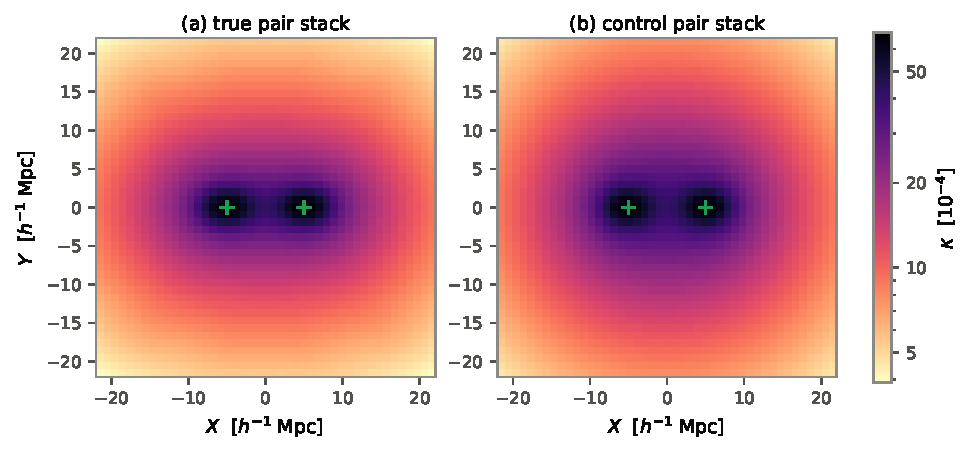
\includegraphics[width=0.9\linewidth]{Figure/sim_pair_vs_control_maps_sep10.pdf}
  \caption{Stacked convergence map from mock galaxy pairs with separation $r_{\perp}=10\,\hinvMpc$ (left) and a control map constructed by superposition of maps of single mock galaxies (right), on a common color scale.
  %that for a controlits
  %unit-amplitude control, Equation~(\ref{eq:control}) (right), on a common
  %color scale.
  %\ZZ{why it is called unit-amplitude?}
  }
  \label{fig:sim_pair_vs_control}
\end{figure*}

\begin{figure*}
  \centering
  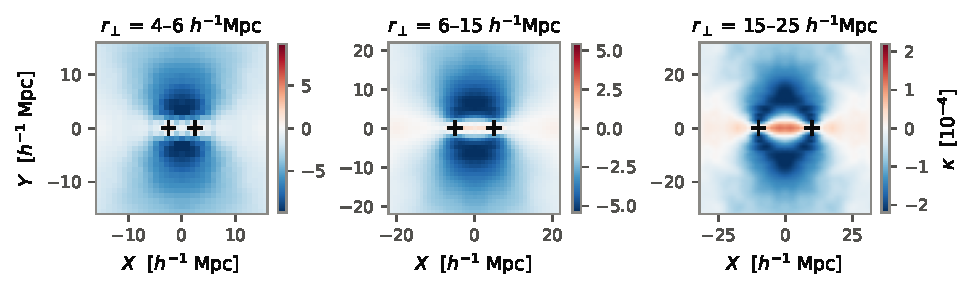
\includegraphics[width=0.9\linewidth]{Figure/sim_quadrupole_diff_maps.pdf}
  \caption{Mock residual maps for pairs with transverse separation $r_{\perp}=5$, $10$, and $20\,\hinvMpc$ (left to right), showing the ridge along the pair axis and the deficit perpendicular to it. Galaxy positions are marked. A residual map is the difference between the stacked map for galaxy pairs and that from superposition of single galaxy map at the pair separation.}
  \label{fig:sim_residual_maps}
\end{figure*}

Figure~\ref{fig:sim_band_profiles} shows the corresponding band profiles. For the $5\hinvMpc$ pairs, the central band becomes negative, which is likely caused by the environment effect of close pairs. The difference between the central and off-center band profile, however, is positive, which shows a bridge between pairs and a declining profile in the outskirt. For the $10\hinvMpc$ and $20\hinvMpc$ pairs, the central band profiles are largely positive. Near the galaxy positions, the residual does not go to zero, as explained above. The bridge excess, calculated within $|X|<0.35$ times the pair separation, is $\left(6.32\pm0.36,\ 4.91\pm0.21,\ 2.18\pm0.12\right)\times10^{-4}$ for the $r_{\perp}=5$, $10$, and $20\,\hinvMpc$ pairs. The decline with separation is consistent with the expectation that the tidal effect and environment effect become less important for pairs at larger separation.

\if{0} {
The
mock bridge excess is
$\left(6.32\pm0.36,\ 4.91\pm0.21,\ 2.18\pm0.12\right)\times10^{-4}$ at
$r_{\perp}=5$, $10$, and $20\,\hinvMpc$. The corresponding $25$-block
jackknife signal-to-noise ratios are $17.7$, $22.9$, and $18.1$.
The decline with separation is consistent with decreases in both the
connected-pair fraction and the mean bridge density. The mock residual also
contains an approximately isotropic component at the galaxy positions and an
anisotropic component along the pair axis.
}\fi
% TODO: quote the mock residual at the halo positions and the midpoint kappa.

\begin{figure*}
  \centering
  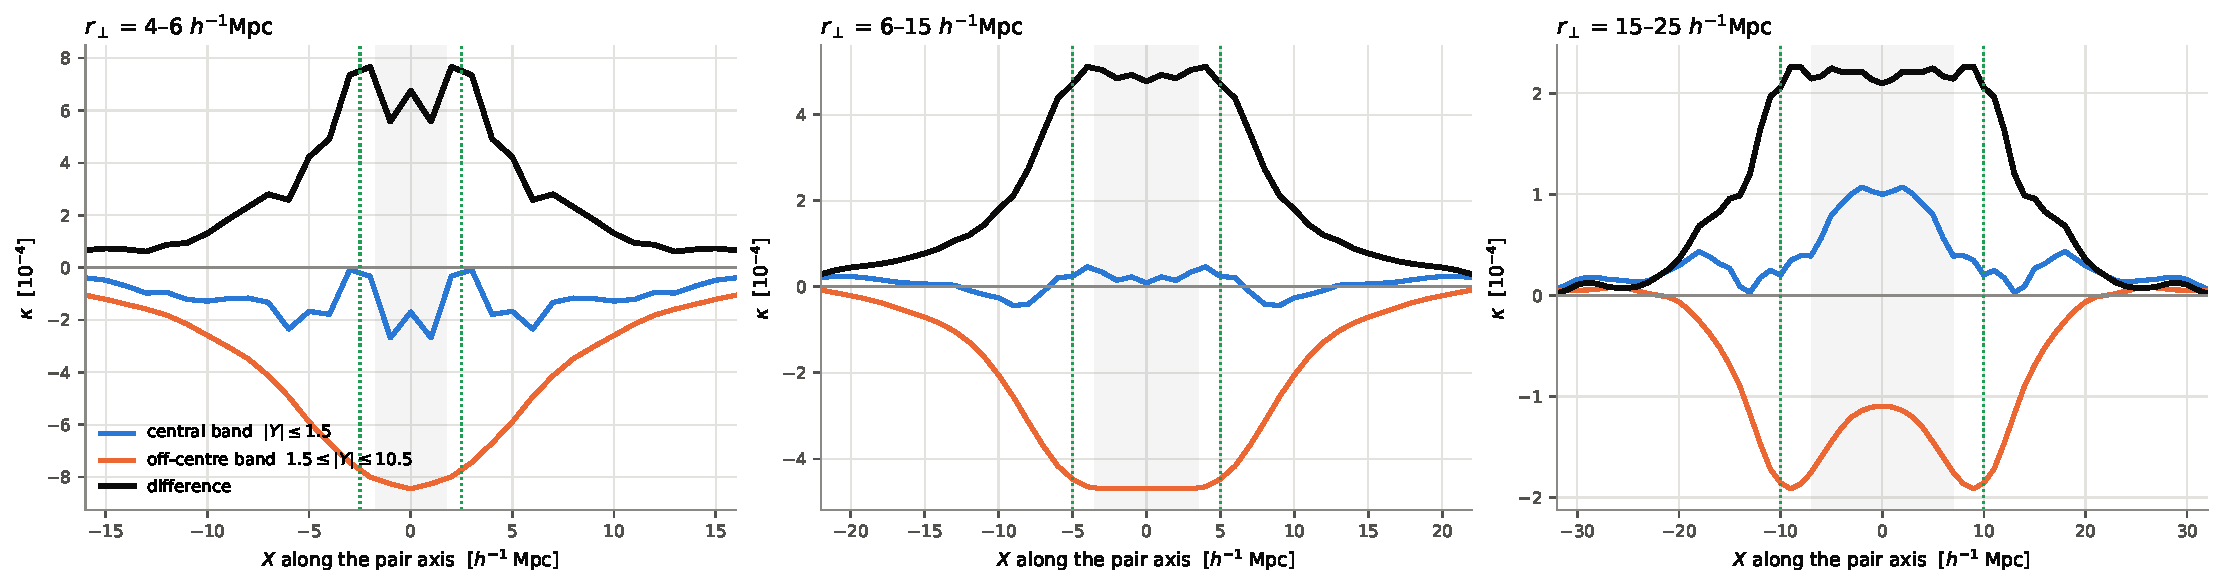
\includegraphics[width=0.9\linewidth]{Figure/sim_band_profiles_all_seps.pdf}
  \caption{Central-band mean profile, off-center-band mean profile, and their difference
  $B(X)$ from the mock residual maps at the three pair separations. The shaded
  window is $|X|\leq0.35\,d$. See text for details.}
  \label{fig:sim_band_profiles}
\end{figure*}

The nonphysical mock pairs show no bridge in any line-of-sight band,
confirming that the control does not itself generate a ridge.
% TODO: per-band residual bridge excess +/- error from nonphysical_pair_test_*.csv.
The line-of-sight sweep supports the production cuts. At
$r_{\perp}=5\,\hinvMpc$ the bridge signal first rises and then falls as the
cut is widened, while at $10\,\hinvMpc$ it falls.
% TODO: completeness / interloper fraction / sensitivity per cut from rpar_scan.csv and los_sweep_summary.csv.

\section{Results}
\label{sec:results}

In this section, we present the measurements of the matter distribution around BOSS CMASS galaxy pairs through cross-correlating galaxy pairs with the Planck CMB lensing map and make comparisons with the reference model from the $N$-body simulation. 

%\subsection{Observed stacks}
\subsection{Measurements of the $\kappa$ map of galaxy pairs and Comparison to Simulations}
\label{sec:obs_stacks}

With $217{,}702$, $459{,}051$, and $1{,}282{,}969$ pairs at $r_{\perp}=5$, $10$, and $20\,\hinvMpc$, we measure the stacked $\kappa$ distribution around them. Figure~\ref{fig:boss_maps} shows the single-galaxy stack and the
three pair stacks, all corrected by subtracting the stacks and random points/pairs and symmetrized according to the reflection symmetry about $X$ and $Y$ axis. All the maps show clear detection of the matter distribution, concentrated at the positions of galaxies.

%The three BOSS samples contain $217{,}702$, $459{,}051$, and $1{,}282{,}969$ pairs at $r_{\perp}=5$, $10$, and $20\,\hinvMpc$. Figure~\ref{fig:boss_maps} shows the corrected single-galaxy stack and the three corrected pair stacks. 
Figure~\ref{fig:obs_vs_sim_maps} compares the
observed and simulated residual maps, obtained by subtracting the control pair maps constructed by superpositions of single galaxy map. 
At distances $\gtrsim 15\hinvMpc$ to the pair center, the observed maps tend to be dominated by noise. At smaller distances, a quadrupole pattern shows up, with a broad $X$-axis-aligned excess and an off-axis deficit, a trend consistent with that expected from simulated maps. The change of the quadrupole pattern with pair separation, e.g., a stronger residual at galaxy positions for $10\hinvMpc$ pairs, also follows that in the simulated maps.

%These residual maps are the observational estimators of filament-associated convergence, but may also contain %imperfectly subtracted halo and environmental contributions. The observed maps contain a broad axis-aligned excess and an off-axis deficit, although both features have low signal-to-noise in the Planck reconstruction.

\begin{figure*}
  \centering
  \includegraphics[width=0.9\linewidth]{Figure/boss_single_and_pair_maps.pdf}
  \caption{Convergence maps from BOSS CMASS single-galaxy stack (left) and pair
  stacks at pair separation $r_{\perp}=5$, $10$, and $20\,\hinvMpc$.}
  \label{fig:boss_maps}
\end{figure*}

\begin{figure*}
  \centering
  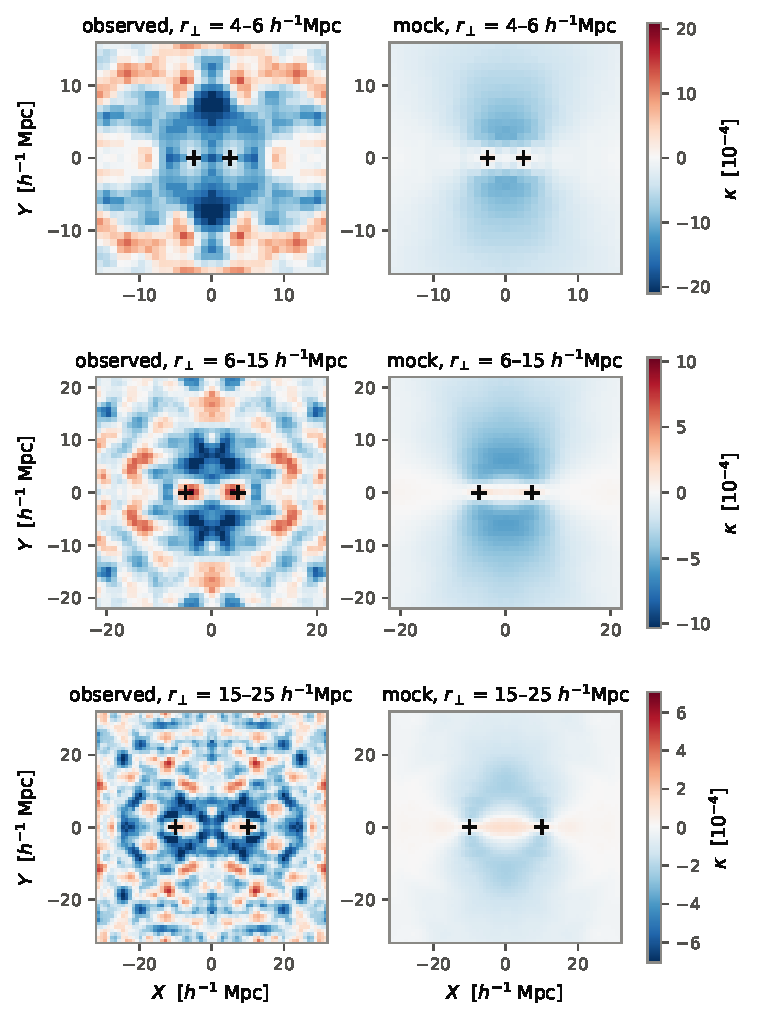
\includegraphics[width=0.7\linewidth]{Figure/obs_vs_sim_quadrupole_maps.pdf}
  \caption{Observed (left) and simulated (right) residual maps for pairs with separation
  $r_{\perp}=5$, $10$, and $20\,\hinvMpc$ (top to bottom), on a common
  color scale per row.}
  \label{fig:obs_vs_sim_maps}
\end{figure*}

%\subsection{Bridge convergence}
%\label{sec:bridge}

Figure~\ref{fig:band_profiles_obs_sim} shows the band profile $B(X)$, the difference between central and off-center average profile defined in Equation~(\ref{eq:band}). Although the observe profiles are noisier, there is general agreement with the simulated profile, with excess in between the pairs. We first computed the bridge excess as the average of $B(X)$ within $|X|<0.35d$ (indicated by the shaded regions in Fig.~\ref{fig:band_profiles_obs_sim}) and estimate the uncertainty based on the jackknife error bars. We find that none of the three bridge excesses exceeds $3\sigma$. The $10\,\hinvMpc$ sample has a positive excess of $2.3\sigma$ and lies $1.4\sigma$ above the mock prediction. The other two measurements are consistent with zero. The results are listed in Table~\ref{tab:bridge}.
%\ZZ{Notes for later discussion: I am somewhat puzzled -- the bridge clearly shows up and the data points within the bridge region are almost coherently positive, but why we have a low significance? Using the 20Mpc/h profile as an example, I see there are 13 points in the bridge region, 7 independent points due to symmetry (did you use the 7 points for the fit?). If I simply use the 7 points, take the error bars as $\sim$3, and neglect the covariance, I would obtain an error bar in the bridge excess at a level of $\sim$3/sqrt(7) $\sim$ 1.13, smaller than 2.22 listed in Table 1. Maybe the covariance is significant? A test can be done by finding the excess only using the diagonal elements of the covariance matrix. (we will have increased number of pairs in the final run, which can likely increase the significance.)}

%Table~\ref{tab:bridge} gives the bridge excess and jackknife error for each sample, together with the mock prediction for the same statistic. Figure~\ref{fig:band_profiles_obs_sim} compares the observed and mock band profiles.

The bridge statistic in Table~\ref{tab:bridge} provides the direct comparison
between the data and mock because both analyses use the same bands, bridge
window, and smoothing. At all three separations, the observational
uncertainties exceed the predicted bridge amplitudes, and the measurements
are consistent with both zero and the mock.

\citet{deGraaff2019} measured
$\bar\kappa=(5.8\pm3.1)\times10^{-4}$ in the bridge region of pairs pooled
over $6$--$14\,\hinvMpc$. Their statistic differs from ours in four ways:
pairs are rescaled to unit separation before stacking, the bridge region is
defined on the rescaled grid, the halo model is fitted to the pair stack in
a $60^\circ$ sector about the direction perpendicular to the pair axis, and
the map is smoothed to $10$ arcmin. Their central value is close to our
$10\,\hinvMpc$ result, but the two estimators differ. Their
sample contains about $2.2$ times as many pairs as our $10\,\hinvMpc$
sample; independent-pair scaling alone would reduce the error by a factor of
$1.5$.
An inverse-variance-weighted combination of our three samples would provide
an approximate comparison, but would still differ from the estimator used by
\citet{deGraaff2019}.
% TODO: quote the pooled value if this comparison is retained.

\begin{table}
  \centering
  \caption{Bridge excess, defined as the average of Equation~(\ref{eq:band})
  over $|X|\leq0.35\,d$, for the three BOSS samples and the mock. Observed
  errors are from the $287$-region delete-one jackknife, with the control
  reconstructed in every realization; mock errors are from the $25$-block
  jackknife. The final column gives the observed-minus-mock difference divided
  by the quadrature sum of the two errors.}
  \label{tab:bridge}
  \begin{tabular}{cccccc}
    \hline
    $r_{\perp}$ & $N_{\rm pairs}$ & Observed & S/N & Mock & Obs.$-$Mock \\
    $[\hinvMpc]$ & & $[10^{-4}]$ & & $[10^{-4}]$ & $[\sigma]$ \\
    \hline
    5  & $217{,}702$   & $5.38\pm9.08$  & $0.6$ & $6.32\pm0.36$ & $-0.1$ \\
    10 & $459{,}051$   & $11.91\pm5.10$ & $2.3$ & $4.91\pm0.21$ & $+1.4$ \\
    20 & $1{,}282{,}969$ & $1.24\pm2.22$  & $0.6$ & $2.18\pm0.12$ & $-0.4$ \\
    \hline
  \end{tabular}
\end{table}

\begin{figure*}
  \centering
  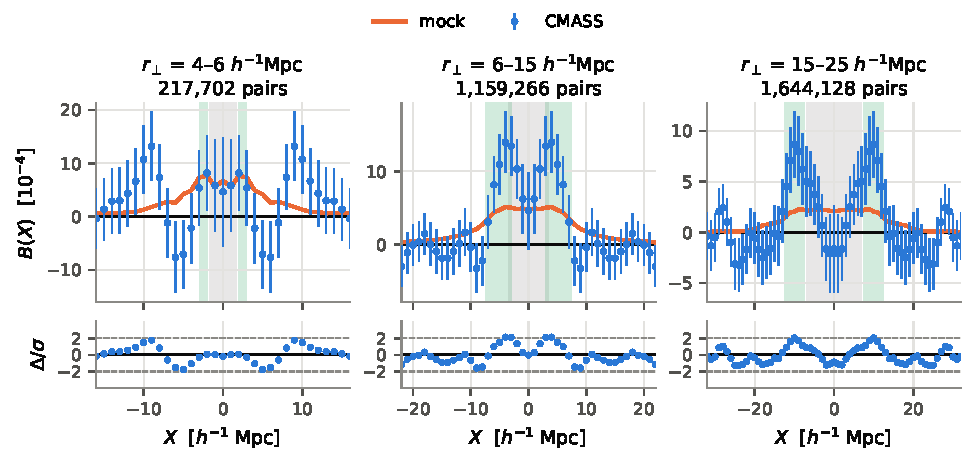
\includegraphics[width=0.9\linewidth]{Figure/band_profiles_obs_vs_sim.pdf}
  \caption{Observed band profiles $B(X)$ with jackknife errors (points) and
  mock profiles at the three pair separations.
  %with box-jackknife errors (shaded) at the three pair separations.
  %Observed errors are from a delete-one jackknife over $287$ sky regions. Mock
  %errors are from the $25$-block box jackknife, with the superposed-singles
  %control held fixed across realizations. 
  The gray region marks the bridge
  window, $|X| \leq 0.35\,d$, with $d$ the pair separation, and the dotted green lines mark the galaxy
  positions. The lower panels show the observed-minus-mock difference in
  units of the observational error, with dashed lines at $\pm2$. Mock pairs
  are selected in the same transverse bins as the BOSS pairs. 
  %The mock errors include statistical scatter within a single realization but not HOD uncertainty.
  }
  \label{fig:band_profiles_obs_sim}
\end{figure*}

%None of the three bridge excesses exceeds $3\sigma$. The
%$10\,\hinvMpc$ sample has a positive excess of $2.3\sigma$ and lies
%$1.4\sigma$ above the mock prediction. The other two measurements are
%consistent with zero.
To see the significance of detecting the central and off-center band profiles, we perform a $\chi^{2}$ test of the compressed $22$-element central and off-center band profile against zero with
the full covariance, which gives $\chi^{2}=35.0$, $20.7$, and $32.4$ for $22$
degrees of freedom (corresponding to nominal $p$ values of $p=0.04$, $0.54$, and $0.07$). The $p=0.04$ result at $5\,\hinvMpc$ applies to the full profile, including bins that contain the galaxies, and therefore does not constitute a bridge detection.
%\ZZ{notes: going to $40\hinvMpc$ seems to be too large, which started to be %dominated by noise. let's consider to reduce the range.}

Fitting the mock residual profile to the observed profile over the full
$22$-element vector using Equation~(\ref{eq:amplitude}) gives
$A=1.47\pm0.36$, $1.07\pm0.49$, and $1.60\pm0.57$, at $4.1$, $2.2$, and
$2.8\sigma$.
At $10$ and $20\,\hinvMpc$, bins around the galaxies contribute $59$ and
$44$ percent of the fitted response, respectively. At $5\,\hinvMpc$, the
$4\,\hinvMpc$ binning places the galaxy positions in the sole bridge bin, so
their contributions cannot be separated. The full-profile amplitude is
therefore not an estimate of the bridge amplitude. Restricting the fit to the
bridge window
$|X|\leq0.35\,d$ gives $A=1.97\pm0.58$, $1.81\pm0.84$, and $0.71\pm0.95$, at
$3.4$, $2.1$, and $0.7\sigma$. These significances differ from the bridge
excesses in Table~\ref{tab:bridge} because the fit treats the central and
off-center bands as separate data elements, whereas the bridge statistic
uses their difference. The $5\,\hinvMpc$ fit still contains the unresolved
galaxy bin, and beam-convolved halo signal can enter the bridge window at all
three separations. We therefore interpret these fits as profile diagnostics,
not bridge detections. Adding a free constant to the full-profile model leaves
the amplitudes unchanged and gives offsets of
$\left(-1.6,\ +0.4,\ +0.2\right)\times10^{-4}$, consistent with zero.

%\subsection{Comparison with the simulation and with previous work}
%\label{sec:compare}

%The bridge statistic in Table~\ref{tab:bridge} provides the direct comparison between the data and mock because both analyses use the same bands, bridge window, and smoothing. At all three separations, the observational uncertainties exceed the predicted bridge amplitudes, and the measurements are consistent with both zero and the mock.



The residual maps also test how well the control describes the paired haloes.
The observed residual map peaks at the galaxy positions at about
$2\times10^{-3}$, compared with $0.9\times10^{-3}$ in the mock.
% CHECK: values from the fit_sim_template.py docstring; confirm from checked-in output.
If confirmed, this difference would imply a larger contrast between paired
and average CMASS galaxies than between paired and average mock galaxies. A
central-only HOD with a soft mass threshold may select pairs differently from
the observed sample, which includes satellites and has a sharper effective
stellar-mass selection. The corrected single-galaxy profile also lies below
the matched mock prediction at large radius.
% CHECK: fit_sim_template.py docstring; compare_boss_mock_profile.py retracted earlier significance values.
These comparisons constrain the isotropic residual from which the
axis-aligned signal is separated. They do not directly measure the bridge
statistic, which subtracts the off-center band in Equation~(\ref{eq:band}).
% TODO: compare corrected single profiles in the 10--20, 15--25, and 20--40 h^-1 Mpc bands with jackknife errors.

%\citet{deGraaff2019} measured $\bar\kappa=(5.8\pm3.1)\times10^{-4}$ in the bridge region of pairs pooled over $6$--$14\,\hinvMpc$. Their statistic differs from ours in four ways: pairs are rescaled to unit separation before stacking, the bridge region is defined on the rescaled grid, the halo model is fitted to the pair stack in a $60^\circ$ sector about the direction perpendicular to the pair axis, and the map is smoothed to $10$ arcmin. Their central value is close to our $10\,\hinvMpc$ result, but the two estimators differ. Their sample contains about $2.2$ times as many pairs as our $10\,\hinvMpc$ sample; independent-pair scaling alone would reduce the error by a factor of $1.5$. An inverse-variance-weighted combination of our three samples would provide an approximate comparison, but would still differ from the estimator used by \citet{deGraaff2019}.
% TODO: quote the pooled value if this comparison is retained.

%A $95$ percent upper limit on the bridge excess can be converted to surface density using $\Sigma_{\rm crit}$ and subsequently to linear mass densityalong the bridge.
% \ZZ{ add this once we do comparison with Epps\&Hudson}
% TODO: compute the upper limits and compare them with Epps & Hudson (2017) and de Graaff et al. (2019).

\subsection{Robustness tests}
\label{sec:robust}

We perform additional analyses to test the robustness of our results.

\paragraph{Smoothing.} Figure~\ref{fig:smoothing_scan} compares the observed results with 
$8$- and $6$-arcmin (FWHM) smoothing at all three separations and with $4$-arcmin  smoothing at $5$ and $10\,\hinvMpc$. The bridge signal-to-noise values for
$8$, $6$, and $4$ arcmin smoothing are $(0.6,1.2,2.2)$ at $5\,\hinvMpc$ and
$(2.3,2.4,1.1)$ at $10\,\hinvMpc$. At $20\,\hinvMpc$, the values with $8$- and
$6$-arcmin smoothing are $0.6$ and $0.5$. We retain $8$ arcmin as the common
smoothing scale and do not tune it separately for each separation.

\begin{figure}
  \centering
  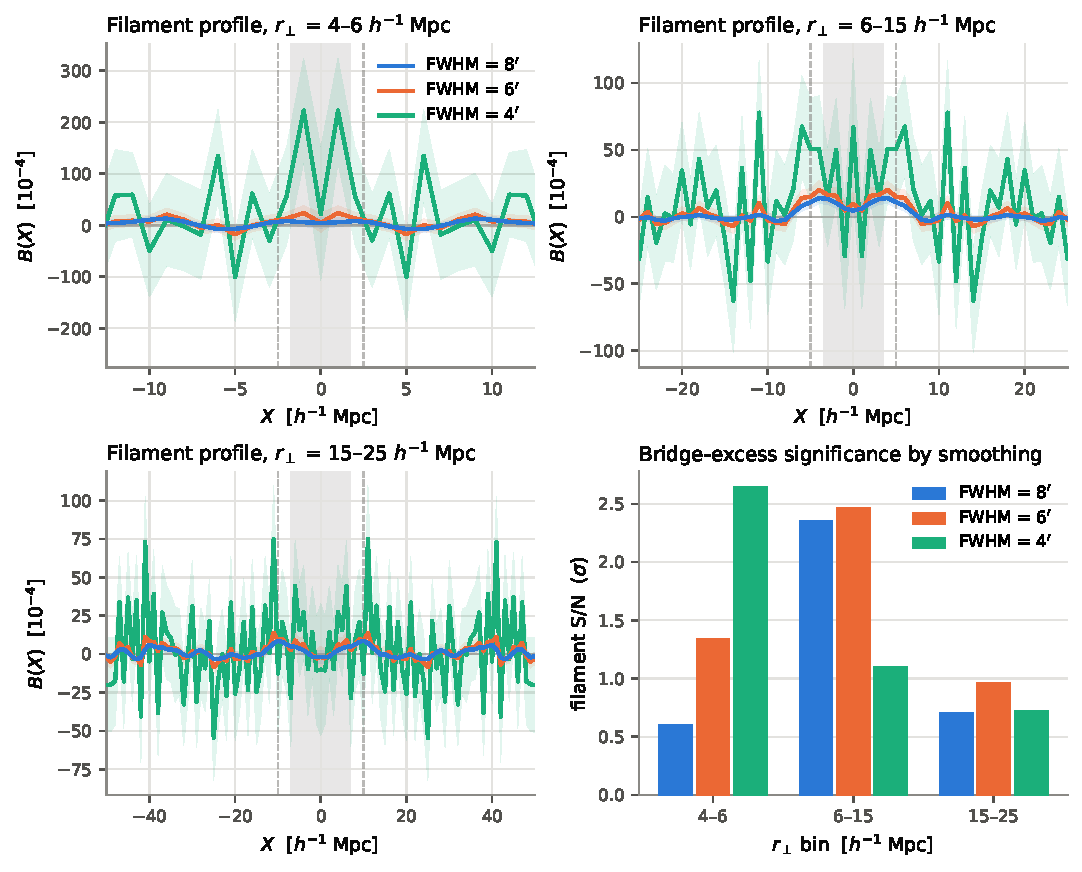
\includegraphics[width=\linewidth]{Figure/filament_snr_vs_smoothing.pdf}
  \caption{Observed bridge profiles and signal-to-noise with there
  smoothing FWHM values. The $4$-arcmin smoothing stack is unavailable at
  $20\,\hinvMpc$.}
  \label{fig:smoothing_scan}
\end{figure}

\paragraph{Weighting.} We have not yet quantified the effect of removing the
lensing-efficiency weight from the single-galaxy stacks.
% TODO: report the changes in the control and bridge excess.
%Combining the two caps with equal weight, rather than as a joint stack, produced the apparent dip found in earlier versions of the analysis.
%\ZZ{I think the joint stack is the way to go.}
% TODO: report the shift in the corrected single profile at 20 h^-1 Mpc.

\paragraph{Random-pair sample.} Replacing the full random catalog by a
10 percent subsample shifts the $10\,\hinvMpc$ bridge excess by
$5\times10^{-4}$, comparable to the measured signal. We therefore use the
full random catalog. % CHECK: combine_filament_jackknife.py docstring.

\paragraph{Fitted control.}
% UNVERIFIED: align this description with band_core_tail_control.py and add checked-in results.
As an alternative to the unit-amplitude control, we split the single-galaxy
profile into core and tail components and fit their amplitudes outside the
pair. In the mock, this procedure drives the bridge excess to zero at all
three separations, whereas the unfitted control recovers the bridge present
in the simulation. The fitted control therefore absorbs axis-aligned signal,
so we do not use it for the fiducial measurement.
% TODO: quote mock and observed bridge excess under the fitted control beside the unfitted values.

\medskip
\medskip

As a whole, by cross-correlating CMASS galaxy pair wth the Planck CMB lensing map, we detect the matter distribution around galaxy pairs at the three pair separations. Comparing to the control pair map, we find the expected quadrupole pattern in the residual matter distribution around galaxy pairs. There is hint of stretched matter (filaments) along the pair connection line, while their significance needs to be further examined by increasing the size of the galaxy pair sample.

\section{Summary and Discussion}
\label{sec:discussion}

In this work, we use the BOSS CMASS galaxy sample and Planck CMB lensing map to probe the matter distribution (dominated by dark matter) around galaxy pairs with a stacking analysis. We have stacked the Planck 2018 lensing convergence map around $217{,}702$,
$459{,}051$, and $1{,}282{,}969$ BOSS CMASS galaxy pairs at transverse
separations of $5$, $10$, and $20\,\hinvMpc$,
subtracted a control built from the galaxies' own single-galaxy stack, and
measured a residual bridge statistic that is sensitive to filament-associated
convergence between the galaxies. We applied the same signal estimator to a
CMASS-like mock built from the BigMDPL $N$-boday simulation, which provides a
$\Lambda$CDM reference prediction for this statistic. We retain the term
``residual'' because the estimator may also contain incompletely subtracted
halo and environmental contributions.

In the residual map, which shows the difference between the matter distribution around true galaxy pairs and that around control pairs (from superposition of single galaxy stacks), a quadrupole pattern is revealed, with excess around the pair connection line and deficit around the perpendicular bisector. It is the first time that this pattern has been discovered in observation. Such a pattern is consistent with the expectation from the simulation model. It is a manifestation of the gravitational interaction between galaxy or halo pairs. Tidal interaction tends to make the matter distribution stretched around the pair connection line and squashed around the perpendicular bisector direction. For models without dark matter, such as the Modified Newtonian dynamics (MOND; \citealt{Milgrom1983}), the gravitational effect comes from the concentrated distribution of baryonic matter in galaxies, which would be hard to produce the observed quadrupole pattern here. 

The quadrople pattern is not seen in \citet{deGraaff2019} with a similar CMB lensing stacking analysis. This may be related to their construction of the control pair $\kappa$ map. In stead of superposition of the $\kappa$ profile around single galaxies, they derive their control map effectively from averaging the pair $\kappa$ in certain range. Such a control map tends to suppress the relatively weak quadrupole pattern. The weak lensing analysis of matter distribution around galaxy pairs in \citet{EppsHudson2017} does not reveal the quadrupole pattern, either. It may be buried in the noise or systematics in the weak lensing analysis. As a comparison, their filament detection results are not supported by \citealt{Xia2020}, with an increased sample of source galaxies for weak lensing.

We construct a band profile from the residual map by taking the difference between the average profile near the pair connection line and the offset from the connection line in the perpendicular direction. The band profile serves to quantify the appearance of filaments. In the band profile of each pair separation, there appears to be a coherent excess between the two galaxies, signaling the filament. The amplitude of the excess broadly agrees with the simulation model. When the jackknife covariance is accounted for, we find that the excess lacks statistical significance if we exclude the region affected by the halo subtraction. In Appendix~\ref{sec:appendix}, we list the lessons learned from our analysis. With an increased size of pair sample, we hope to further investigate the filament signal.

%\textbf{Prospects.} 
The CMB lensing noises appear to dominate the error budget in our analysis.
Increasing the number of pairs
should reduce the statistical error until correlations in the convergence
map become limiting. A wider separation bin would provide the most direct
gain with Planck, at the cost of smearing the separation dependence. A larger
gain requires a less noisy convergence map. The ACT DR6 lensing map covers
$9400\,\mathrm{deg}^{2}$ and overlaps part of the CMASS footprint, but the
overlap and noise improvement relevant to this estimator remain to be
quantified. % CHECK: quote overlap area and noise ratio; add ACT DR6 citation.
The Simons Observatory and CMB-S4 should provide further improvements in CMB
lensing sensitivity. % CHECK: add forecast citations and quantify for this statistic.
The SPT-3G overlap with CMASS should also be quantified before deciding
whether it is useful for this measurement. Scaling our errors by a measured
noise ratio would give a forecast for the mock bridge at $10\,\hinvMpc$ with
the present pair sample. % TODO: report the forecast S/N.
Combining the convergence stack with the
thermal Sunyaev--Zel'dovich stack of the same pairs, as \citet{deGraaff2019}
did, would then constrain the gas temperature of the bridge as well as its
mass. Finally, subsets of the CMASS pairs overlap the HSC, DES, and KiDS shape
catalogs. A joint galaxy-shear and CMB-lensing analysis would test the bridge
using two independent source planes. % CHECK: quantify overlap and add survey citations. 

\begin{comment}
\section{Theoretical Expectation}

\subsection{Method}

\todo[inline]{method of computing $\kappa$ from simulation, single galaxies, galaxy pairs; including equations.}

When we see the extra lensing between galaxies, we must determine how much of it comes from the filament and the residual coming from the galaxy halos’ own overlap in the middle. To claim a filament signal we first must predict how much lensing two isolated halos would put there on their own, and then subtract that. This prediction is what we call the template, or control, and the simulation is where we build it and find out whether it works. The simulation is necessary because in the real sky there is no way to check the filament/halo distribution between the two galaxies, while in the simulation there is. We use the BigMDPL box, 2500 $\hinvMpc$ on a side at redshift 0.547, identify the dark matter halos in it, and place galaxies in them tuned to match the number density of the real BOSS CMASS sample. Because we can compute the lensing directly from the simulated matter, we know the true answer for every test we run. 

\begin{equation}
\Sigma(r_{p,i})
= \frac{\sum_{k=1}^{N_h} N_{p,k}\left(|r_p-r_{p,i}|<\Delta r_p/2\right) M_{p,{\rm eff}} /N_h}{\pi [(r_{p,i}+\Delta r_p/2)^2-(r_{p,i}-\Delta r_p/2)^2]}  - \frac{N_{p,{\rm tot}} M_{p,{\rm eff}}}{L^2},
\label{eqn:sim_Sig}
\end{equation}

Equation~(\ref{eqn:sim_Sig}) is an example

\subsection{Characterizing $\kappa$ Map from Galaxy Pairs}

Before measuring anything on the sky, we use the simulation to gauge how much filament is actually present after the control is subtracted. 

Figure~\ref{fig:sim_pair_vs_control_maps_sep10} shows the simulated pair stack at r\_perp = 10 $\hinvMpc$ beside its single-based control. The control is made up of two copies of the measured single-galaxy profile placed at $\pm r_\perp / 2$ along the pair axis (with no fitted parameters). This is the map we would expect if each galaxy carried its own isolated halo and nothing lay between. On the shared color scale the two panels look almost identical–highlighting the difficulty of the measurement. The filament is a small residual between two large and similar maps, so the accuracy of the control matters a lot. 

Subtracting the control from the observed map leaves a clever pattern at all three separations (Figure~\ref{fig:sim_quadrupole_diff_maps}): positive along the pair axis between the galaxies, and negative above and below it. The residual also contains the fact that a halo with a companion is not identical to an isolated halo–but its shape is what makes the measurement possible. A filament lies along the axis while the deficit sits off it. 

Instead of working with a full 2D residual map, we collapse it into two profiles along the pair axis (Figure~\ref{fig:sim_band_profiles_all_seps}): a central band covering $|Y| \le 1.5 \, \hinvMpc$, where a filament would lie, and an off-center band covering $1.5 \le |Y| \le 10.5 \, \hinvMpc$, bracketing it. Their difference cancels anything that varies slowly with Y, including any large-scale offset the two bands share, and turns the map into one number per position along the axis. Rows at the band boundaries are given fractional weights according to how much of each row falls inside the band, so the statistic does not depend on where the pixel edges land. 

The single-galaxy band profile is not a single object. We split it at $r_{\text{c}} = 3 \, \hinvMpc$ into a core, the measured profile inside that radius, and a tail, which is a Gaussian continuation matched to the profile's value and slope at the boundary $\sigma = 3.23 \, \hinvMpc$). These two pieces contribute very differently depending on separation. At the midpoint between the galaxies, the core supplies 100\% of the control at $r_\perp = 5$, 71\% at $r_\perp = 10$, and only 3.6\% at $r_\perp = 20$. At small separations the signal is dominated by the galaxies’ own inner profiles, and at large separations it is made of their outskirts. A control with one amplitude cannot get both regions right, so we fit the core and tail amplitudes separately, using only the region outside the pair where no filament can contribute. 

Fitted this way, the paired halos come out to: $A_{\text{core}} = 1.06$, $1.02$, $1.01$ and $A_{\text{tail}} = 0.96$, $1.02$, $1.05$ at $r_\perp = 5, 10, 20$. The residual left in the bridge is $-1.56 \pm 1.13$, $+1.23 \pm 1.94$, and $+0.50 \pm 1.30$ ($\times 10^{-4}$), with errors from a delete-one jackknife over 25 blocks of the simulation box. The simulation does not predict a large signal in this statistic–a useful expectation to carry into the observational results. 

\begin{figure}
   \centering
    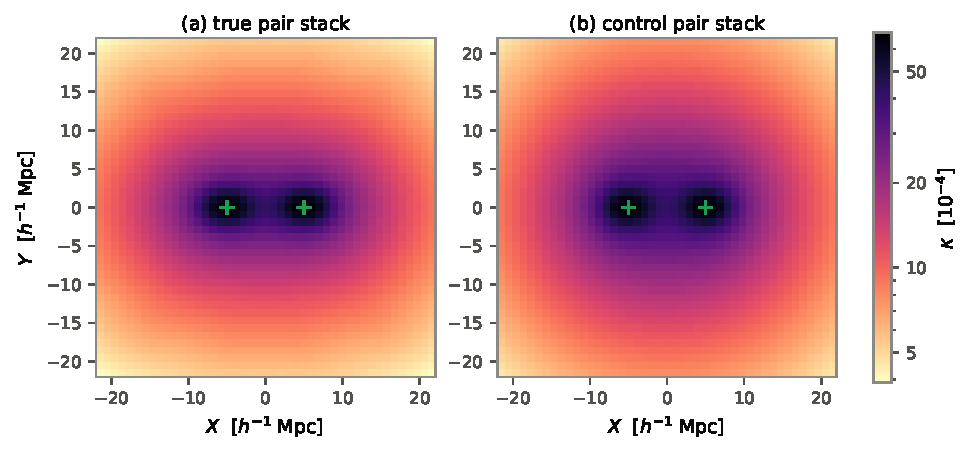
\includegraphics[width=0.45\linewidth]{Figure/sim_pair_vs_control_maps_sep10.pdf}
    \caption{
    Figure to show true pair $\kappa$ map (a) and single-based control $\kappa$ map (b), use $10\hinvMpc$ pairs as an example
    }
    \label{fig:sim_pair_vs_control_maps_sep10}
\end{figure}

Figure to show the difference (a-b) map to illustrate the quadrupole pattern, one row with 5, 10, and 20$\hinvMpc$ from left to right

\begin{figure}
   \centering
    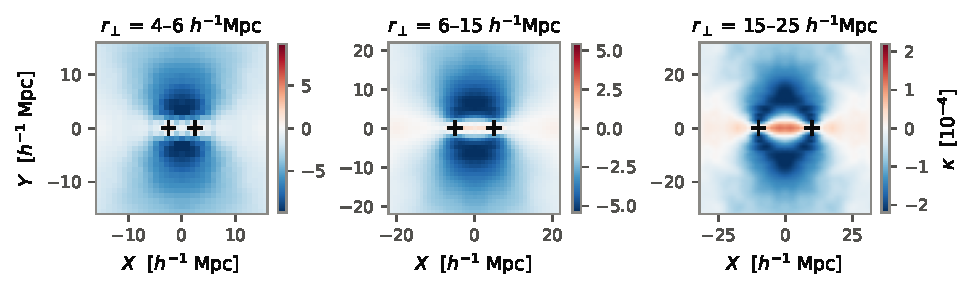
\includegraphics[width=0.45\linewidth]{Figure/sim_quadrupole_diff_maps.pdf}
    \caption{
    Figure to show the difference (a-b) map to illustrate the quadrupole pattern, one row with 5, 10, and 20$\hinvMpc$ from left to right
    }
    \label{fig:sim_quadrupole_diff_maps}
\end{figure}

Figure to show the central-band, off-center-band, and difference based on the (a-b) map, 5, 10, 20$\hinvMpc$, from left to right

\begin{figure}
   \centering
    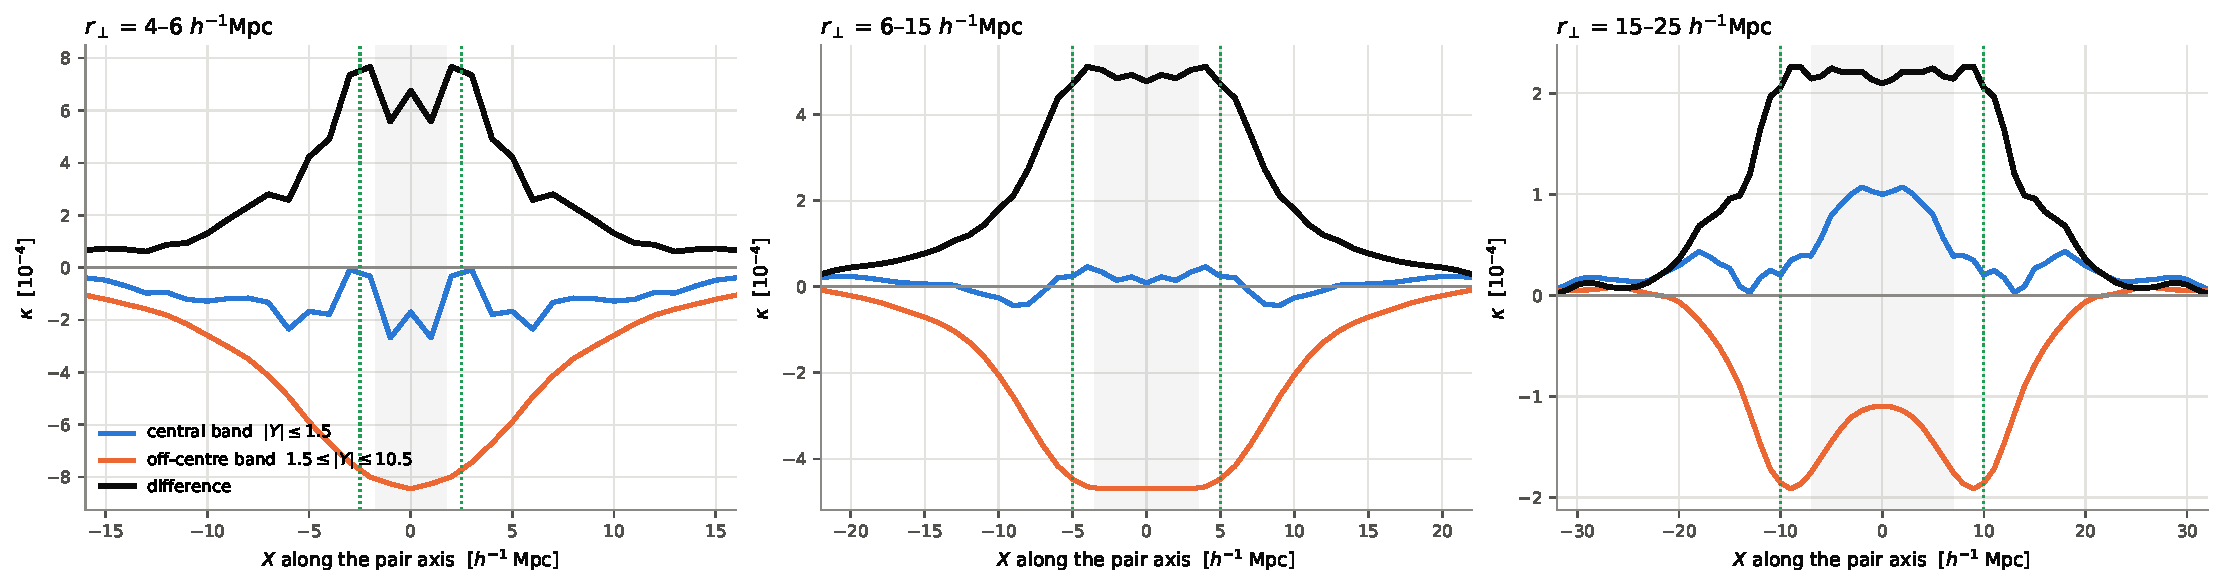
\includegraphics[width=0.45\linewidth]{Figure/sim_band_profiles_all_seps.pdf}
    \caption{
    Figure to show the central-band, off-center-band, and difference based on the (a-b) map, 5, 10, 20$\hinvMpc$, from left to right
    }
    \label{fig:sim_band_profiles_all_seps}
\end{figure}

Figure to show central band profile for single superposition, show the decomposition

\begin{figure}
   \centering
    \includegraphics[width=0.45\linewidth]{Figure/band_core_tail_decomposition.pdf}
    \caption{
    Figure to show central band profile for single superposition, show the decomposition
    }
    \label{fig:footprint_zdist}
\end{figure}

Figure to show 5, 10, 20$\hinvMpc$ measured pair central band vs fitted control pair profiles (3 panels from left to right) , with difference in bottom smaller panel of each top panel

\begin{figure}
   \centering
    \includegraphics[width=0.45\linewidth]{Figure/band_core_tail_fitted_central.pdf}
    \caption{
    Figure to show 5, 10, 20$\hinvMpc$ measured pair central band vs fitted control pair profiles (3 panels from left to right) , with difference in bottom smaller panel of each top panel
    }
    \label{fig:footprint_zdist}
\end{figure}

\section{Measurement Results}

\subsection{Methods}

\todo[inline]{including equations.} We rotate and stack hundreds of thousands of galaxy pairs along the same axis in the same positions to reduce noise and isolate the filament signal. The rotation ensures that each pair’s bridge is aligned and not smeared in a ring. For every pair of galaxies we compute two separations, both in comoving $\hinvMpc$ – r\_perp (separation across the line of sight) and r\_par (separation along the line of sight). A pair enters a sample if r\_perp falls in the chosen bin (4–6, 9–11, or 18–22 $\hinvMpc$) and r\_par is below the cut. A galaxy can appear in more than one pair, and we do not remove these. For each pair we lay down a square grid, 100 $\hinvMpc$ on a side, sampled at 101 × 101 points. That gives exactly 1 $\hinvMpc$ between grid points. The grid is oriented so that X runs along the line joining the two galaxies. The galaxies sit at $X = -r_\perp/2$ and $X = +r_\perp/2$. We find the midpoint and rotation angle, then convert grid points to sky positions by rotating each grid point by $\theta$, dividing by the pair’s comoving distance, and adding to the midpoint’s coordinates, resulting in Galactic longitude and latitude. We work in Galactic coordinates rather than RA/Dec throughout. Each grid point's (l, b) is converted to the HEALPix convention and mapped to the pixel of the Planck map containing it, and that pixel's $\kappa$ value is read off. At nside = 2048 the pixels are about 1.7 arcmin, comfortably finer than the 1 $\hinvMpc$ grid spacing, so no interpolation is needed. The stack is a weighted mean, computed separately for every pixel. The stacked map has four-fold symmetry built into the physics. We average four quadrants: the value at $(+X, +Y)$ is replaced by the mean of $(+X, +Y)$, $(-X, +Y)$, $(+X, -Y)$, and $(-X, -Y)$. Every value in the final map is an average of four measurements of the same physical quantity, which reduces the noise. This is different from symmetrization used for single galaxies, which averages in circular rings. The same procedure is run on pairs drawn from the random catalogs — same separation cuts, same rotation, same weighting. The randoms contain survey footprints but no real structure, so subtracting it leaves the galaxy signal. 

\subsubsection{Pair selection}

A pair is defined by two comoving separations, r\_perp, perpendicular to the line of sight, and r\_par, along the line of sight. r\_perp is what we bin on: 4–6, 9–11, 18–22 $\hinvMpc$, called the 5, 10, and 20 $\hinvMpc$ samples. r\_par has to be small for a physically connected pair ($\le 5 \, \hinvMpc$ at $5$; $\le 10 \, \hinvMpc$ at $10$ and $20$). 

\subsubsection{Joint N+S estimator}
\todo[inline]{no need to talk about what wrong before, just describe what's currently implemented, also check the statement about random catalogs}
BOSS CMASS covers two disconnected parts of the sky, the larger Northern one and a smaller Southern one. They have to be combined into a single measurement. The earlier profiles stacked each region separately and then averaged the two with equal weight, which is the wrong thing to do because the Northern section contains far more galaxies, meaning its measurement is more precise. Weighing the two equally produced a visible artifact–an apparent dip at 20 $\hinvMpc$ that looked like a physical feature but was purely a result of the weighing. The current analysis addresses this problem by stacking every galaxy from both regions into a single running total. Nothing is separated, so the need for averaging is gone. The same applies to random catalogs, which are stacked jointly in the same way, so the galaxy-minus-random subtraction is between two consistently constructed quantities.  

\subsubsection{Spatial jackknife and covariance}

Because we are measuring the sky, the measurement cannot be repeated to see how much it scatters. The delete-one jackknife gets an error from a single dataset instead by dividing the sky into many patches, repeating the whole measurement with one patch removed at a time, and using the scatter across those repeats as the uncertainty. If the answer barely moves each time a patch is dropped, the measurement is robust. The standard $(K-1)/K$ factor converts that scatter into an error, correcting for the fact that the repeats overlap heavily. To build each patch, we utilize the fact that the sky is divided into equal-area HEALPix cells of about 34 square degrees. Cells containing enough galaxies become patch centers; cells only partly covered at the survey’s ragged edge are merged into the nearest neighboring patch, so no galaxy falls outside. This yields 287 patches of roughly equal size that span both the north and the south regions. The stack is accumulated separately for each patch in a single pass, so leaving a patch out means just subtracting its running total from the total. All 287 repeats then cost just as much as one stack. The reported map is galaxies minus randoms. Both galaxies and randoms share a single layout, so every leave-one-out estimate is a valid version of the subtracted map, and the error applies to the quantity reported. The analysis computes the full covariance, not just how much each bin scatters, but how much each pair of bins scatters together, and uses it whenever bins are combined. The full covariance is needed because the profile has many bins along the pair axis, each with its own jackknife error. Combining them as if they were independent would be wrong, because the Planck map is smoothed over about 3.3 $\hinvMpc$ while the bins are 1 $\hinvMpc$ wide, so a single blur spans three bins and neighbouring bins rise and fall together. Finally, the fitted quantities are refitted in every repeat. Any parameter estimated from the data is re-estimated inside each leave-one-out realization rather than fixed at its full-sample value. Holding a fitted parameter leaves its uncertainty out and makes a method appear ten times more precise than it actually is (as determined in one of our control tests). 

Note: Planck’s $\kappa$ map is noise-dominated at these scales. After smoothing, the pixels are not independent anymore (8-arcmin beam is more than three times the size of one pixel), so treating pixels as independent understates the error. 

\subsection{Results}

We apply the estimator fixed in simulation – fitted core+tail control, r\_c = 3 $\hinvMpc$, no additive constant – to BOSS CMASS. The samples contain 217,702, 459,051, and 1,282,969 pairs at $r_\perp = 5$, $10$, and $20$ $\hinvMpc$. NOTE: The $r_\perp = 10$ and $20$ samples use a line-of-sight cut of r\_par $\le 10 \hinvMpc$; the $r_\perp = 5$ sample uses r\_par $\le 5$. All errors come from the 287-patch delete-one jackknife, with every fitted parameter re-fitted inside each realization. 

Figure Z shows the symmetrized single-galaxy stack besides three pair stacks. Figure A compares the observed difference maps with the simulated ones. The observed maps show the same broad quadrupole seen in simulation–excess along the pair axis, deficit above and below–but at much lower signal-to-noise, because the Planck reconstruction is noise-dominated at these scales. 

The core amplitude of the fitted control comes out to close to one at all three separations: $A_{\text{core}} = 0.84 \pm 0.11$, $0.99 \pm 0.13$, and $1.08 \pm 0.11$. Halos in observed pairs are therefore consistent with isolated halos of the same profile, matching the simulation. It is important to note that two things do not match. The tail amplitude is systematically low – $A_{\text{tail}} = 0.78 \pm 0.29$, $0.52 \pm 0.26$, and $0.50 \pm 0.28$, against 0.96–1.05 in simulation – meaning the real single-galaxy profile falls off faster at a larger radius than the mock does. The fitted core width is also narrower, $\sigma = 2.90 \hinvMpc$ observed against 3.23 predicted, about 10\% smaller. Both point the same way: the mock galaxies sit in slightly more extended halos than the real CMASS sample. 

The bridge residual between galaxies after subtracting the fitted control

\begin{table}[ht]
    \centering
    \caption{Mean bridge convergence and its significance, measured on the
             central band of the pair stack after subtracting the fitted
             core+tail control. The bridge window is $|X| \leq r_\perp/4$.
             Errors are from the 287-region delete-one jackknife, with every
             fitted parameter re-fitted in each realization.}
    \label{tab:bridge}
    \begin{tabular}{ccc}
        \hline
        $r_\perp$ [$\hinvMpc$] & Bridge $\kappa$ [$10^{-4}$] & Significance \\
        \hline
        5  & $+1.74 \pm 11.29$ & $0.15\sigma$ \\
        10 & $+8.94 \pm 7.45$  & $1.20\sigma$ \\
        20 & $+4.39 \pm 4.60$  & $0.95\sigma$ \\
        \hline
    \end{tabular}
\end{table}

All three are consistent with zero. The values are positive, and the $r_\perp = 10$ point is the largest, but none reaches the level at which we would claim a measurement. Testing the individual bins against zero with a $\chi^2$ and the full covariance does not change the conclusion. No separation exceeds $1.9\sigma$ once the excluded region around each galaxy is at least one beam width wide.

To ensure the control is accurate, we checked outside the fitted region and discerned that the residual is consistent with zero at all three separations, so there's no evidence that the control under or over-subtracts. The scatter of the residual away from the halos is 3.27, 3.24, and 2.04, comparable to the quoted bridge errors, which confirms that the errors reflect real map noise rather than fit instability. The residuals at the halo positions themselves are $+3.37 \pm 4.72$, $+12.46 \pm 5.56$, and $+0.45 \pm 3.82$. The $r_\perp = 10$ halo residual is the one mild outlier, at $2.2\sigma$. 

The errors are large because of the Planck map. Measuring the same bridge window on the unfitted central band with no control and no fitted parameters yields errors of $(10.57, 7.35 \text{ and } 4.84) \times 10^{-4}$, within 7\% of the quoted values at every separation. Fitting the control is effectively free. 

The simulation predicts a bridge of $-1.56 \pm 1.13$, $+1.23 \pm 1.94$, and $+0.50 \pm 1.30$ in the same statistic. The observations are consistent with these values, but the observational errors are 4-9 times larger, so the measurement cannot distinguish the signal from zero. For context, de Graaff et al. (2019) measured the same quantity on the same lens sample and source, reporting $\kappa = (5.8 \pm 3.1) \times 10^{-4}$ at $1.9\sigma$. Their central value is comparable to ours at $r_\perp = 10$ ($+8.94$), but their error is 2.4 times smaller, largely because they pool all pairs from 6 to 14 $\hinvMpc$ into one rescaled measurement rather than resolving separation as we do. 


Figure show stacked symmetrized single, 5, 10, 20 pair $\kappa$
maps (left-right), 4 panels

\begin{figure}
   \centering
    \includegraphics[width=0.45\linewidth]{boss_single_and_pair_maps.pdf}
    \caption{
    Figure show stacked symmetrized single, 5, 10, 20 pair $\kappa$
    maps (left-right), 4 panels
    }
    \label{fig:footprint_zdist}
\end{figure}

Figure to show (a-b) maps, left observed, right theoretical, three rows for 5, 10, and 20$\hinvMpc$

\begin{figure}
   \centering
    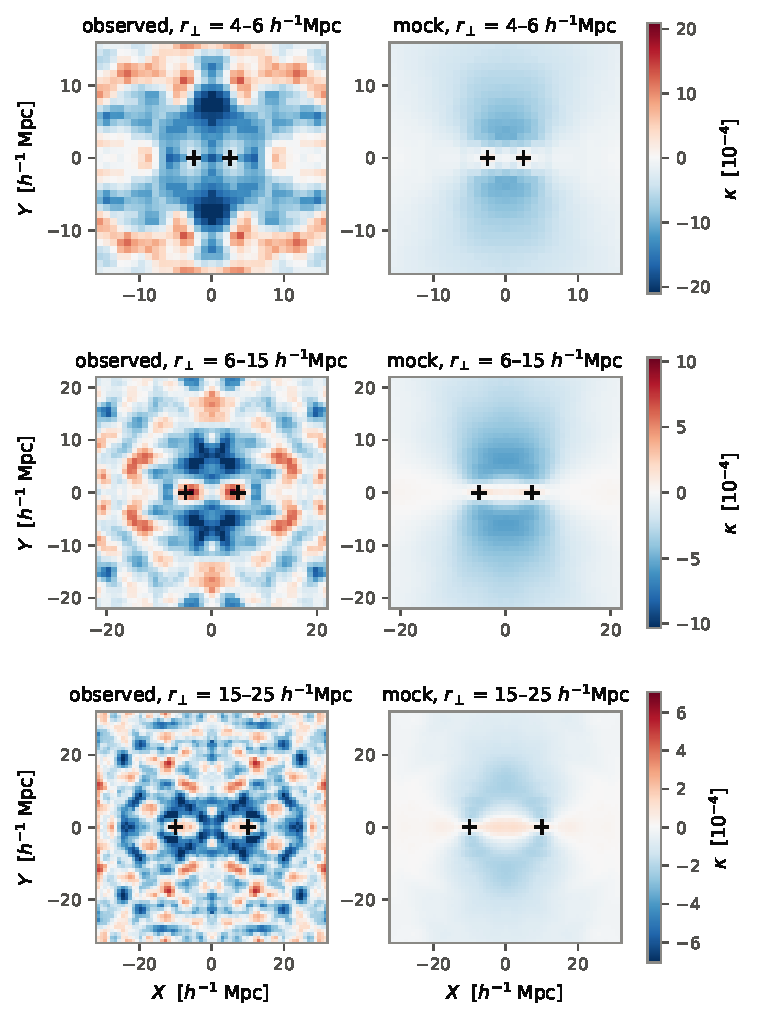
\includegraphics[width=0.45\linewidth]{Figure/obs_vs_sim_quadrupole_maps.pdf}
    \caption{
    Figure to show (a-b) maps, left observed, right theoretical, three rows for 5, 10, and 20$\hinvMpc$
    }
    \label{fig:footprint_zdist}
\end{figure}

Figure to show central band profile for observed single superposition, show the decomposition

\begin{figure}
   \centering
    \includegraphics[width=0.45\linewidth]{Figure/boss_band_core_tail_decomposition.pdf}
    \caption{
    Figure to show central band profile for observed single superposition, show the decomposition
    }
    \label{fig:footprint_zdist}
\end{figure}

Figure to show 5, 10, 20$\hinvMpc$ observed pair central band vs fitted control observed pair profiles (3 panels from left to right) , with difference in bottom smaller panel of each top panel

\begin{figure}
   \centering
    \includegraphics[width=0.45\linewidth]{Figure/boss_band_core_tail_central.pdf}
    \caption{
    Figure to show 5, 10, 20$\hinvMpc$ observed pair central band vs fitted control observed pair profiles (3 panels from left to right) , with difference in bottom smaller panel of each top panel
    }
    \label{fig:footprint_zdist}
\end{figure}

need some thoughts on comparing observation and theory, we may have more figures

\section{Summary and Discussion} 
\label{sec:summary}

We stacked the Planck lensing map on 217,702, 459,051, and 1,282,969 CMASS
galaxy pairs at transverse separations of 5, 10, and 20 $h^{-1}$ Mpc,
subtracted a control built from the galaxies' own single-galaxy stack, and
measured what was left between them.

\textbf{We do not detect a filament.} The bridge is consistent with zero at all
three separations, at $0.15\sigma$, $1.20\sigma$, and $0.95\sigma$. This does
not change when the individual profile bins are tested against zero with the
full covariance instead of averaged, nor when the quadrupole is measured
directly from the difference maps.

\textbf{The limit is the map, not the method.} Removing the control entirely
and measuring the same window on the raw band changes the error by less than
7\%. Fitting the control is effectively free, so no improvement to the template
can shrink the error bar. Only more pairs or a less noisy convergence map can.

\textbf{The control behaves.} The fitted core amplitude is consistent with one
at every separation, so halos in observed pairs look like isolated halos of the
same profile, as in the simulation. Outside the fitted region the residual is
consistent with zero, and non-physical pairs return no signal.

\textbf{Two mismatches with the mock are worth noting.} The fitted tail
amplitude is low ($0.50$--$0.78$ against $0.96$--$1.05$ predicted) and the core
is about 10\% narrower than predicted ($\sigma = 2.90$ against $3.23$
$h^{-1}$ Mpc). Both point the same way: the mock galaxies sit in slightly more
extended halos than the real CMASS sample. This affects the shape of the
control, not the conclusion, but it suggests the HOD could be tuned on the
lensing profile rather than the number density alone.

\textbf{One methodological result generalises beyond this work.} When removing
the halo positions from a bridge measurement, the excluded region must be at
least as wide as the smoothing scale. Excluding only $\pm 1$ $h^{-1}$ Mpc,
against a Planck beam of 3.3 $h^{-1}$ Mpc, left enough halo signal inside the
window to produce an apparent $2.4\sigma$ bridge that vanished once the
exclusion reached a full beam width.

\textbf{Improvements.} Because the error is dominated by map noise, it falls as
the sample grows, so widening the separation bins is the most direct gain
available with existing data. Beyond that, the deeper convergence maps from
ACT, SPT-3G, and eventually CMB-S4 offer far lower noise over the CMASS
footprint, and a measurement of this kind is likely to become possible there
before it becomes possible with Planck. Using a single line-of-sight cut across
all three separation bins would also make the samples directly comparable.

\end{comment}

\begin{acknowledgments}
We are grateful to Prof.\ Zheng Zheng for his guidance throughout this
project, for many discussions that shaped the analysis, and in particular
for proposing the subset test that established the sample-variance origin
of the outer-profile offset in the simulated single-galaxy stack. We thank
Dr.\ Di He for [helpful discussions on / a careful reading of an early draft
of / advice on] this work. % CHECK: state Dr. He's contribution specifically
Any remaining errors are our own.

%Funding for SDSS-III has been provided by the Alfred P.\ Sloan Foundation,
%the Participating Institutions, the National Science Foundation, and the
%U.S.\ Department of Energy Office of Science. The SDSS-III web site is
%\url{http://www.sdss3.org/}. SDSS-III is managed by the Astrophysical
%Research Consortium for the Participating Institutions of the SDSS-III
%Collaboration. % Paste the full institution list required by SDSS-III here.

%This work is based on observations obtained with Planck
%(\url{http://www.esa.int/Planck}), an ESA science mission with instruments
%and contributions directly funded by ESA Member States, NASA, and Canada.
%We use the Planck 2018 lensing products from the Planck Legacy Archive.

%The CosmoSim database used in this paper is a service by the
%Leibniz-Institute for Astrophysics Potsdam (AIP). The MultiDark database
%was developed in cooperation with the Spanish MultiDark Consolider Project
%CSD2009-00064. The authors gratefully acknowledge the Gauss Centre for
%Supercomputing e.V.\ (\url{www.gauss-centre.eu}) and the Partnership for
%Advanced Supercomputing in Europe (PRACE, \url{www.prace-ri.eu}) for
%funding the MultiDark simulation project by providing computing time on the
%GCS Supercomputer SuperMUC at Leibniz Supercomputing Centre
%(LRZ, \url{www.lrz.de}).

This research made use of \textsc{astropy}, \textsc{healpy}, \textsc{numpy},
\textsc{scipy}, and \textsc{matplotlib}. % add \citep keys if your journal wants software cited
\emph{Declaration of AI use.} Generative AI tools were used in this project.
This declaration states what they were used for, what they were not used for,
and when.

\emph{Tools and versions.} All AI assistance was obtained through Claude Code,
Anthropic's command-line coding assistant. The models used, as recorded in the
co-authorship trailers of the project's version-control history, were Claude
Opus 4.6 (February 2026), Claude Opus 5, including its 1M-context configuration
(August and September 2026), and Claude Fable 5.1 (September 2026).
% CHECK: add any other AI tool used outside this repository. If none, say so.

\emph{Work completed without AI assistance.} The measurement method of this
paper was developed before any AI tool was used on the project. Between
2025 July 17 and 2026 February 5, the first author wrote the original analysis
in Jupyter notebooks and committed it in 59 revisions: the construction of the
convergence maps, the galaxy-pair catalogs, the stacking and symmetrization
procedure, the control subtraction, and the first error estimates. Bugs found
and fixed in that period, including an error in the Mpc$/h$ conversion and a
comparison of the equatorial and Galactic coordinate implementations, were
diagnosed by the first author. The research question, the choice to look for
filaments between CMASS pairs in the Planck lensing map, and the design of the
control were proposed and refined in discussion with Prof.\ Zheng Zheng and
Dr.\ Di He. These notebooks are preserved in the project repository under
\texttt{legacy/}.

\emph{Work in which AI assisted.} From 2026 February onward, AI assistance was
used at three stages.

First, software. The notebooks were restructured into the current command-line
pipeline with AI assistance, and much of that code---catalog loading, pair
selection, the stacking routines, the jackknife covariance estimation, and the
plotting scripts---was corrected with AI assistance. Debugging was a continuous
part of this: corrections made with AI assistance include an out-of-memory failure
in the random-catalog loader, a normalization error in the control-pair map, and a
half-pixel error in the centering of the stacking grid.

Second, verification. AI was used to audit the code and the intermediate
results. Two errors that affected numbers previously written into this draft
were found this way: a mismatch between the transverse separation bin used for
the mock and that used for the data (Section~\ref{sec:sim}), and an
inconsistency between the bridge-band definitions applied to the mock and to
the observation (Section~\ref{sec:method}). Both were corrected before
submission.

Third, the manuscript. Sections of this report were polished with AI assistance
from the authors' outlines, results, and notes, and were then revised more by the
authors. AI was also used for a spelling-convention pass.

\emph{What AI was not used for.} No numerical result reported here was produced
by a language model. Every value in the text, tables, and figures is an output
of the analysis code running on the public BOSS, Planck, and MultiDark data
described in Section~\ref{sec:data}, and can be recomputed from the archived
pipeline. AI was not used to generate, alter, or select data; the catalogs and
maps are public and unmodified. The physical model was not chosen by AI: the
cosmology is Planck 2018 and the halo occupation form is that of
\citet{White2011}, adopted on the advice of Prof.\ Zheng Zheng. No AI-edited
code or text entered the repository or this report without being read and
accepted by the authors, who are responsible for all of its content, including
any remaining errors.

\emph{Timing and frequency.} AI assistance was used between 2026 February and
2026 September, in two concentrated periods: the restructuring of the pipeline
in 2026 February, and the verification in 2026 August
and September. No AI tool was used on this project before 2026 February.

\end{acknowledgments}

\appendix

\section{Tests and findings related to the analysis}
\label{sec:appendix}

In this appendix, we describe additional tests and the lessons learned from the analysis.

\textbf{No bridge excess exceeds $3\sigma$, and the data do not distinguish
between the mock prediction and zero.} The bridge excesses have
signal-to-noise ratios of $0.6$, $2.3$, and $0.6$ at the three separations. A
test of the full compressed profile gives nominal $p$-values of $0.04$,
$0.54$, and $0.07$.
The $p=0.04$ result at $5\,\hinvMpc$ includes bins containing the galaxies and
is not evidence for a bridge. The mock predicts bridge excesses of
$\left(6.32\pm0.36,\ 4.91\pm0.21,\ 2.18\pm0.12\right)\times10^{-4}$ in the
same statistic. These amplitudes are smaller than the observational errors
at all three separations. At $10\,\hinvMpc$, the measurement is $2.3\sigma$
from zero and $1.4\sigma$ from the mock prediction.
% TODO: 95 percent upper limits as Sigma and linear mass density.
The $2.3\sigma$ excess at $10\,\hinvMpc$ has a similar nominal significance
to the $1.9\sigma$ result of \citet{deGraaff2019}, but the two measurements
use different estimators and should not be interpreted as measurements of
the same quantity.

\textbf{Binning by separation resolves the predicted trend but reduces
sensitivity.} Unlike \citet{deGraaff2019}, we bin pairs by separation on a
fixed comoving grid rather than rescaling and pooling them. The predicted
bridge decreases by a factor of three from $5$ to $20\,\hinvMpc$, so a pooled
measurement combines structures with different expected amplitudes. Dividing
the sample increases the error in each bin, and none yields a $3\sigma$
bridge excess. Pooling our three bins with inverse-variance weights gives
$\left(3.05\pm1.99\right)\times10^{-4}$, or $1.5\sigma$. This provides only an
approximate comparison with \citet{deGraaff2019}, whose estimator rescales and
pools pairs before stacking. The quoted error also neglects cross-covariance among our
three samples, which share a footprint and can share galaxies, and is not a
formal uncertainty on the combined measurement.

\textbf{The Planck map appears to set the present sensitivity.} The
contribution from control uncertainty can be quantified by applying the same
band statistic before control subtraction.
% TODO: quote the exact change from the committed pipeline (the 7 percent figure came from the fitted-control analysis).
If this comparison changes the error only marginally, the error budget is
dominated by Planck reconstruction noise within the bridge window, and
refinements to the control alone will not substantially reduce the error.
Treating pixels as independent would have understated
the error by a factor of $2.2$ to $2.6$, % CHECK
showing that the covariance between pixels must be retained.

\textbf{The unit-amplitude control prevents the halo model from absorbing
axis-aligned signal.}
We use a control with no fitted parameters. In the mock, the unit-amplitude
control recovers a clear bridge with the expected decline with separation. A
preliminary test in which the core and tail amplitudes are fitted outside the
pair drives the bridge excess toward zero at every separation.
% UNVERIFIED: fitted-control outputs are not in the repo
Regions along the pair axis contain pair-aligned large-scale structure on both
sides of the galaxies. Fitting the control in these regions can therefore
absorb part of the bridge signal. Nonphysical mock pairs, with
line-of-sight separations of
$20$--$120\,\hinvMpc$, provide a separate null test of whether the
unit-amplitude control generates a ridge. % TODO: values

\textbf{The residual near the galaxies tests the control and the mock.}
The observed residual map reaches about $2\times10^{-3}$ at the galaxy
positions, compared with $0.9\times10^{-3}$ in the mock. % CHECK
Possible contributions to this difference include the halo-mass and
environmental selection of paired galaxies, the absence of satellites from
the mock, and the different redshift weighting of the single-galaxy and pair
stacks. The corrected BOSS single-galaxy profile may also fall below the mock
at large radii. % CHECK
These effects can change the isotropic residual, which the band difference
suppresses to first order, and the halo signal that leaks
into the bridge window. They motivate two extensions of the mock: including
satellites and testing the HOD against the measured single-galaxy lensing
profile as well as the number density.

\textbf{The bridge window must account for beam leakage.} The window
$|X|\leq0.35\,d$ ends $0.15\,d$ from each halo center: $0.75\,\hinvMpc$ at
$d=5$, $1.5\,\hinvMpc$ at $d=10$, and $3\,\hinvMpc$ at $d=20$. The smoothing
FWHM is $3.3\,\hinvMpc$. At a given $X$, the central band lies closer to the
halo than the off-center band, so an isotropic
halo residual leaks into the band difference with a positive sign. In an
earlier version of this analysis, excluding only $\pm1\,\hinvMpc$ around
each halo produced an apparent $2.4\sigma$ bridge that vanished once the
exclusion reached a full beam width. % CHECK: from the earlier (uncommitted) analysis; confirm the numbers or drop the sentence
At $5\,\hinvMpc$, excluding a full smoothing width around each galaxy leaves
no bridge window, so the bridge cannot be separated from halo leakage. We use
this bin mainly as a consistency check on the two larger-separation bins and
interpret the $5\,\hinvMpc$ mock statistic as bridge plus halo leakage.
% TODO: quote the mock leakage estimate (B(X) with the filament removed, or with randomized pair orientations)
More generally, a pair-stacking analysis must either separate its bridge
window from the halo centers by a scale comparable to the smoothing FWHM or
calibrate the leakage using a simulation with matched smoothing and halo
selection.

\textbf{The line-of-sight cut trades completeness against contamination.}
We test this cut on the mock rather than adopting the
$5$--$6\,\hinvMpc$ value used previously. The redshift-space sweep evaluates
completeness and interloper fractions at cuts of $5$, $10$, $20$, and
$30\,\hinvMpc$.
% TODO: report the completeness and interloper fractions.
We adopt
$5\,\hinvMpc$ for the closest pairs and $10\,\hinvMpc$ for the other two
samples.
% CHECK: reconcile los_contamination_table.py and rpar_scan.py before submission.
The gain over a uniform $5\,\hinvMpc$ cut remains to be quantified in the
mock. % TODO: report the gain.
If this gain is small, a common cut would simplify comparisons
among separation bins with little loss of sensitivity.


\bibliography{ref}{}
\bibliographystyle{aasjournalv7}

\end{document}
